\documentclass[preprint2]{aastex}
%DIF LATEXDIFF DIFFERENCE FILE
%DIF DEL old.tex   Wed Aug 26 16:30:49 2026
%DIF ADD new.tex   Wed Aug 26 18:06:33 2026
\usepackage{amsmath,amstext}
\usepackage{tikz,xspace}
\usepackage{fancyvrb}
\usetikzlibrary{shapes.geometric,arrows,positioning,calc}
\usepackage[breaklinks,colorlinks,citecolor=blue,linkcolor=magenta]{hyperref}
\usepackage[all]{hypcap} %Links go to figures. This breaks deluxetables; use \capstartfalse \capstarttrue around deluxetables to fix it.
%\usepackage{deluxetable}

\newcommand{\colr}[1]{{\bf \textcolor{red}{[#1]}}}
\newcommand{\brg}{Br$\gamma$\xspace}
\newcommand{\sa}{Sgr~A*\xspace}
\newcommand{\msun}{M_{\odot}\xspace}
\newcommand{\mhsix}{M_{\rm h,6}\xspace}
\newcommand{\Sim}{\sim\!}
\newcommand{\tn}[1]{\tablenotemark{#1}}
\newcommand{\mr}[1]{\multirow{2}{*}{#1}}
\newcommand{\tabspace}{\rule{0pt}{1.0em}}

\defcitealias{Li:2015a}{G. Li et al. 2015}
\defcitealias{Li:2015b}{S. Li et al. 2015}
%DIF < \defcitealias{Guillochon:2014a}{GMR14}
%DIF PREAMBLE EXTENSION ADDED BY LATEXDIFF
%DIF PREAMBLE EXTENSION ADDED BY LATEXDIFF
\RequirePackage{xcolor} %DIF PREAMBLE
\RequirePackage{soul} %DIF PREAMBLE
\RequirePackage{ulem} %DIF PREAMBLE
\normalem %DIF PREAMBLE
 %DIF PREAMBLE
\definecolor{addhl}{rgb}{1.0,0.93,0.45} %DIF PREAMBLE
\definecolor{addtx}{rgb}{0.05,0.30,0.05} %DIF PREAMBLE
\definecolor{deltx}{rgb}{0.72,0.10,0.10} %DIF PREAMBLE
 %DIF PREAMBLE
\sethlcolor{addhl} %DIF PREAMBLE
 %DIF PREAMBLE
% Added text: highlighted in yellow, dark green ink. %DIF PREAMBLE
% \hl cannot span math or fragile content, so fall back to colour alone there. %DIF PREAMBLE
\providecommand{\DIFaddtex}[1]{{\protect\color{addtx}\protect\uwave{#1}}} %DIF PREAMBLE
\providecommand{\DIFdeltex}[1]{{\protect\color{deltx}\protect\sout{#1}}} %DIF PREAMBLE
 %DIF PREAMBLE
% Block-level (float/environment) markers %DIF PREAMBLE
\providecommand{\DIFaddbegin}{} %DIF PREAMBLE
\providecommand{\DIFaddend}{} %DIF PREAMBLE
\providecommand{\DIFdelbegin}{} %DIF PREAMBLE
\providecommand{\DIFdelend}{} %DIF PREAMBLE
\providecommand{\DIFaddFL}[1]{{\protect\color{addtx}#1}} %DIF PREAMBLE
\providecommand{\DIFdelFL}[1]{{\protect\color{deltx}#1}} %DIF PREAMBLE
\providecommand{\DIFaddbeginFL}{} %DIF PREAMBLE
\providecommand{\DIFaddendFL}{} %DIF PREAMBLE
\providecommand{\DIFdelbeginFL}{} %DIF PREAMBLE
\providecommand{\DIFdelendFL}{} %DIF PREAMBLE
%DIF END PREAMBLE EXTENSION ADDED BY LATEXDIFF %DIF PREAMBLE
%DIF HYPERREF PREAMBLE %DIF PREAMBLE
\providecommand{\DIFadd}[1]{\texorpdfstring{\DIFaddtex{#1}}{#1}} %DIF PREAMBLE
\providecommand{\DIFdel}[1]{\texorpdfstring{\DIFdeltex{#1}}{}} %DIF PREAMBLE
%DIF AMSMATHULEM PREAMBLE %DIF PREAMBLE
\makeatletter %DIF PREAMBLE
\let\sout@orig\sout %DIF PREAMBLE
\renewcommand{\sout}[1]{\ifmmode\text{\sout@orig{\ensuremath{#1}}}\else\sout@orig{#1}\fi} %DIF PREAMBLE
\makeatother %DIF PREAMBLE
%DIF LISTINGS PREAMBLE %DIF PREAMBLE
\RequirePackage{listings} %DIF PREAMBLE
\lstdefinelanguage{DIFcode}{ %DIF PREAMBLE
%DIF DIFCODE_BOLD %DIF PREAMBLE
  % unfortunately \bfseries cannot be combined with ttfamily without extra packages %DIF PREAMBLE
  % also morecomment=[il] is broken as of v1.5b of listings at least %DIF PREAMBLE
  % workaround: plot in white with tiny font %DIF PREAMBLE
  % morecomment=[il]{\%DIF\ <\ }, %DIF PREAMBLE
  moredelim=[il][\color{white}\tiny]{\%DIF\ <\ }, %DIF PREAMBLE
  moredelim=[il][\sffamily\bfseries]{\%DIF\ >\ } %DIF PREAMBLE
} %DIF PREAMBLE
\lstdefinestyle{DIFverbatimstyle}{ %DIF PREAMBLE
	language=DIFcode, %DIF PREAMBLE
	basicstyle=\ttfamily, %DIF PREAMBLE
	columns=fullflexible, %DIF PREAMBLE
	keepspaces=true %DIF PREAMBLE
} %DIF PREAMBLE
\lstnewenvironment{DIFverbatim}[1][]{\lstset{style=DIFverbatimstyle,#1}}{} %DIF PREAMBLE
\lstnewenvironment{DIFverbatim*}[1][]{\lstset{style=DIFverbatimstyle,showspaces=true,#1}}{} %DIF PREAMBLE
\lstset{extendedchars=\true,inputencoding=utf8}

%DIF END PREAMBLE EXTENSION ADDED BY LATEXDIFF

\begin{document}

\shorttitle{A Self-Sustaining Black Hole Engine Powered by the Disruptions of Stars}

\shortauthors{Guillochon and Loeb}

\title{A Self-Sustaining Black Hole Engine Powered by the Tidal Disruptions of Stars}

\author{James Guillochon\DIFdelbegin %DIFDELCMD < \altaffilmark{1,2} %%%
\DIFdelend \DIFaddbegin \altaffilmark{1} \DIFaddend and Abraham Loeb\DIFdelbegin %DIFDELCMD < \altaffilmark{1}%%%
\DIFdelend \DIFaddbegin \altaffilmark{2}\DIFaddend }
\DIFdelbegin %DIFDELCMD < \altaffiltext{1}{Harvard-Smithsonian Center for Astrophysics, The Institute for Theory and
%DIFDELCMD < Computation, 60 Garden Street, Cambridge, MA 02138, USA}
%DIFDELCMD < \altaffiltext{2}{Einstein Fellow}
%DIFDELCMD < %%%
\DIFdelend \DIFaddbegin \altaffiltext{1}{Gentleman astrophysicist}
\altaffiltext{2}{Harvard-Smithsonian Center for Astrophysics, The Institute for Theory and
Computation, 60 Garden Street, Cambridge, MA 02138, USA}
\DIFaddend 

\email{jguillochon@cfa.harvard.edu}

\begin{abstract} 
It has been recently suggested that tidal disruption events (TDEs) prefer host galaxies that are undergoing (or have undergone) a burst of recent star formation, which suggests that a minority of galaxy types may be responsible for the majority of events. Because the disruptions occur in galaxies that are intrinsically rare, their individual rates may be as high as $10^{-2}$~gal$^{-1}$~yr$^{-1}$, which is difficult to achieve through stellar relaxation alone. The molecular clouds that surround nuclear clusters play an important role in setting the stellar relaxation rate and thus the rate of tidal disruption, and can provide a path for increasing the rate above what stellar relaxation can provide. We show that (post-)starburst galaxies, for which nearby prototypes are observed to contain significant molecular gas reservoirs, are likely in a self-sustaining cycle where an enhancement in the rate of tidal disruption results in an increase in the density of the surrounding molecular clouds due to momentum injection from the unbound debris of tidal disruptions. \DIFdelbegin \DIFdel{This suggests that }\DIFdelend \DIFaddbegin \DIFadd{Solving for the steady state, we find that the disruption rate saturates at $3 \times 10^{-3}$--$4 \times 10^{-2} (M_{\rm h}/10^{6} M_{\odot})^{-1/6}$~yr$^{-1}$, tens to hundreds of times the canonical rate, the range reflecting whether the clouds form a spherical belt or a flattened disk. In either case the black hole is surrounded by parsec-scale clouds of density $10^{4}$--$10^{5}$~cm$^{-3}$ closely resembling those of the Milky Way's Central Molecular Zone, with a total mass of a few $\times 10^{5} M_{\odot}$ comparable to the molecular disks now resolved around nearby active nuclei. Because stars fed to the black hole from a disk return their unbound debris to the plane they came from, the feedback is self-focusing. The state is self-limiting: stellar collisions cap the rate, and the engine consumes its fuel on a timescale of $10^{8}$--$10^{9}$~yr, comparable to the ages of post-starburst hosts. Because the equilibrium nucleus is heavily obscured ($A_{\rm V} \sim 50$), we predict that the highest-rate nuclei are systematically missing from optically selected samples and should instead be found in the infrared, and that }\DIFaddend current and future \DIFdelbegin \DIFdel{tidal disruption }\DIFdelend surveys should target galaxies \DIFdelbegin \DIFdel{that contain central gas }\DIFdelend \DIFaddbegin \DIFadd{containing central }\DIFaddend reservoirs of the densest molecular gas \DIFdelbegin \DIFdel{that are }\DIFdelend accompanied by low levels of AGN activity.
\end{abstract}

\keywords{black hole physics --- galaxies: active --- gravitation}

\bigskip
\noindent\fbox{\parbox{0.95\columnwidth}{\small
\textbf{How to read this document.} This is a marked-up comparison between the
original unfinished draft and the revised manuscript, produced with
\texttt{latexdiff}.
\smallskip

{\color{addtx}\uwave{Text added in the revision appears in green with a wavy underline.}}
\smallskip

{\color{deltx}\sout{Text removed from the original appears in red with a strikethrough.}}
\smallskip

Unmarked text is unchanged. The figures \texttt{mom-rates.pdf},
\texttt{dominance.pdf} and \texttt{domratio.pdf} were regenerated from the
corrected equations and are \emph{not} marked as changed here, because their
filenames did not change; the versions shown are the new ones.
\texttt{engine-diagram.pdf} is unchanged. The bibliography was rebuilt from
scratch and so is not diffed meaningfully.
}}
\bigskip

\DIFdelbegin \section{\DIFdel{Notes}}
%DIFAUXCMD
\addtocounter{section}{-1}%DIFAUXCMD
%DIFDELCMD < 

%DIFDELCMD < \begin{itemize}
\begin{itemize}%DIFAUXCMD
%DIFDELCMD < \item %%%
\item%DIFAUXCMD
\DIFdel{https://arxiv.org/abs/1802.00973
}%DIFDELCMD < \item %%%
\item%DIFAUXCMD
\DIFdel{https://arxiv.org/abs/1805.12132
}
\end{itemize}%DIFAUXCMD
%DIFDELCMD < \end{itemize}
%DIFDELCMD < 

%DIFDELCMD < %%%
\DIFdelend \section{Introduction}\DIFaddbegin \label{sec:intro}
\DIFaddend 

Black holes grow by feeding on gas delivered to them from their surroundings; this gas is either delivered to them in the form of low-density flows that funnel through an extended accretion disk structure \citep{Salpeter:1964a}, or by the disruptions of gravitationally self-bound structures such as stars and planets \citep{Rees:1988a}. In both cases, the black hole emanates light and mass (in the form of outflows) which can feed energy and momentum into its neighborhood \citep{Fabian:2012a, Metzger:2015a, Jiang:2016b}. The majority of the energy released by an accreting black hole is in the form of light unless the light is trapped within the accretion flow, which occurs when the accretion rate exceeds the Eddington limit $L_{\rm Edd} \equiv 4 \pi G M_{\rm h} m_{\rm p} c / \sigma_{\rm T}$; above this limit, jets and outflows carry away similar amounts of energy.

\begin{figure*}[t]
\centering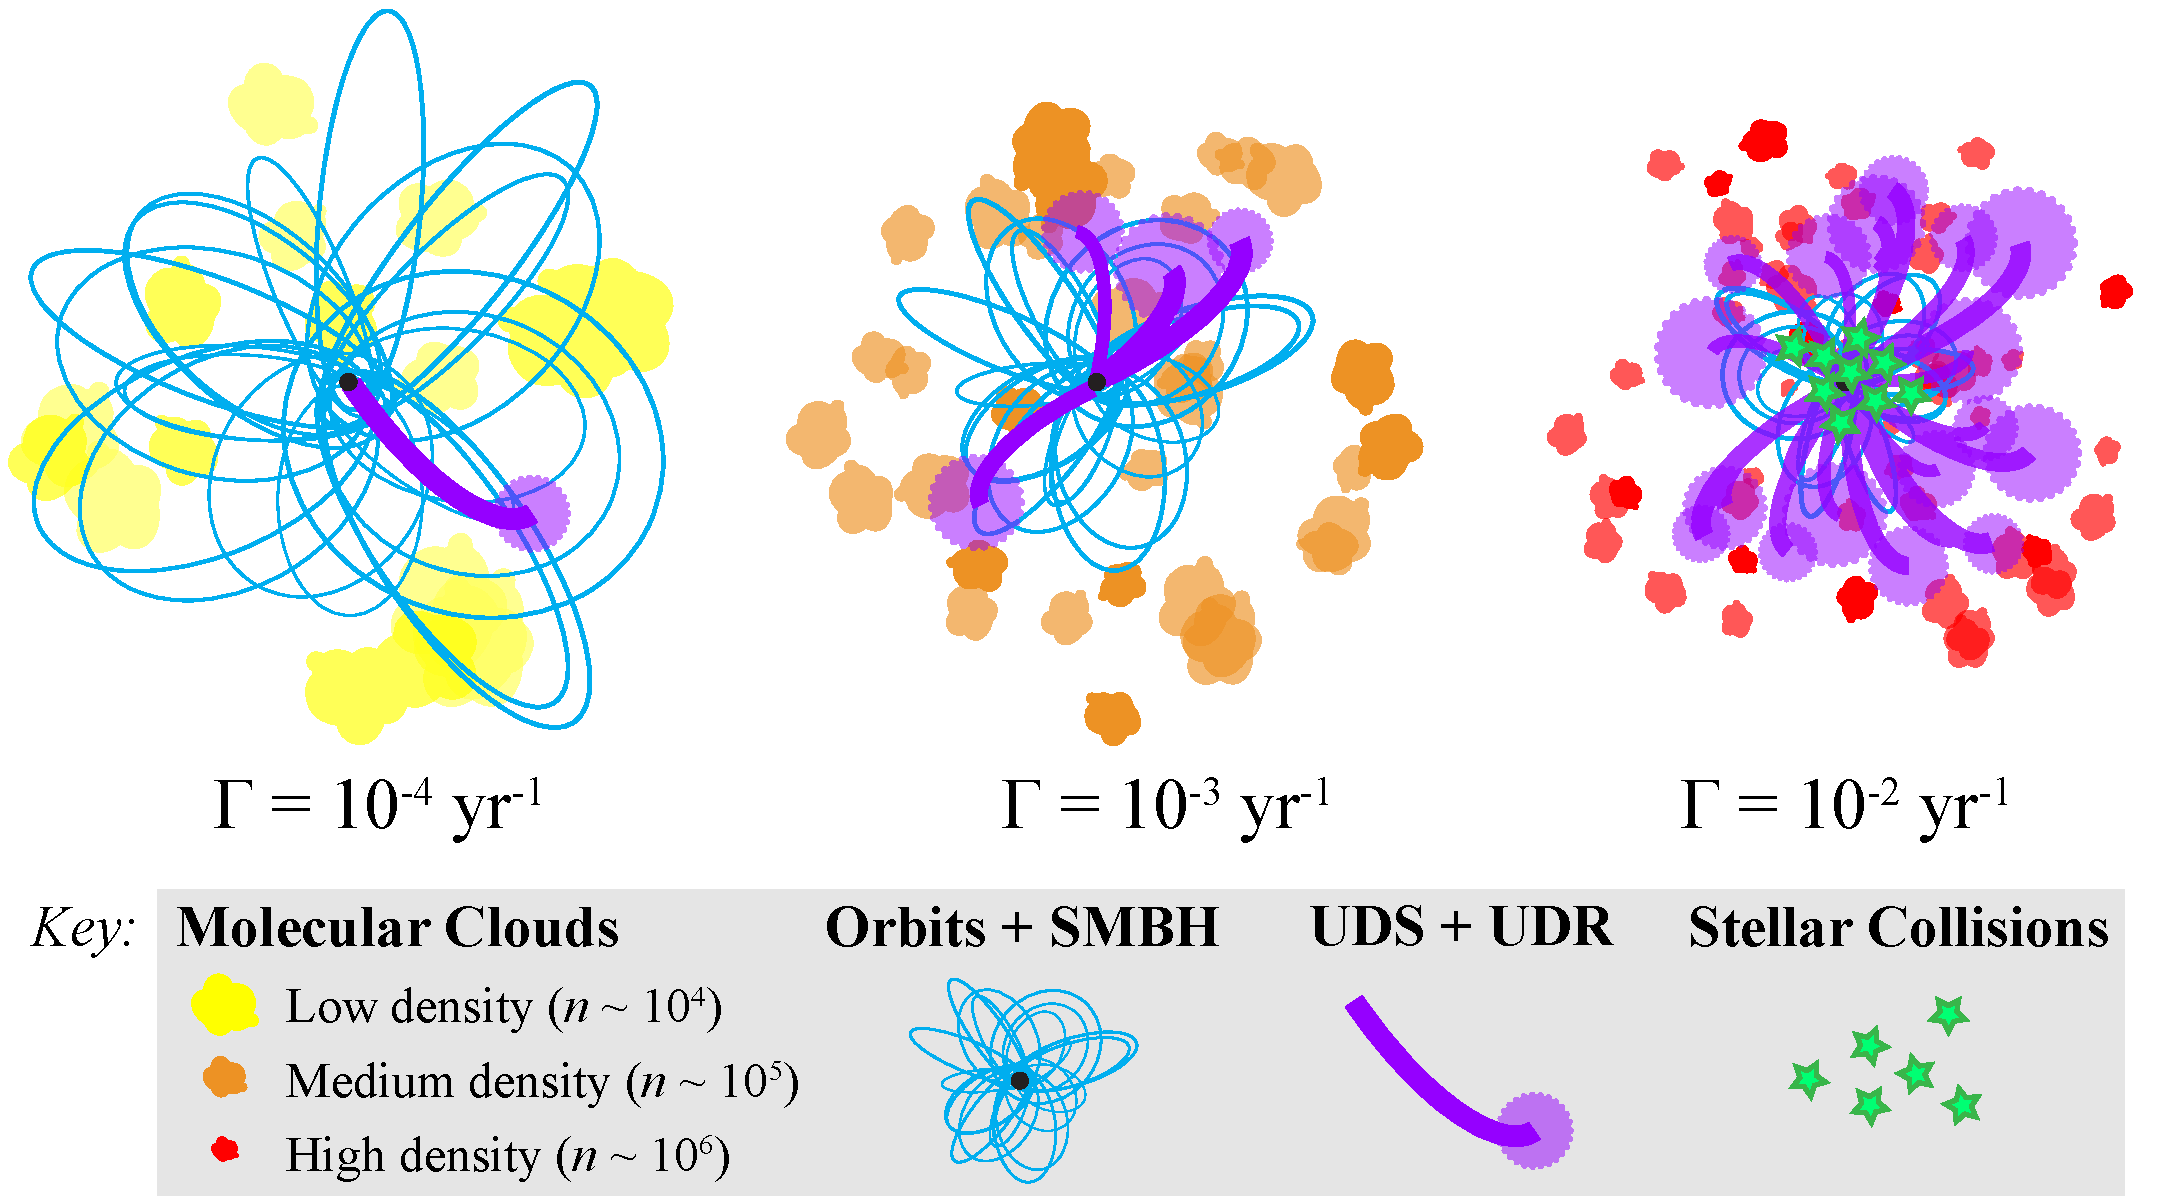
\includegraphics[width=0.8\linewidth,clip=true]{engine-diagram.pdf}
\caption{Evolution of the nuclear cluster and surrounding dense molecular clouds as the rate of disruptions increases, with the left panel showing the conditions arising from stellar relaxation alone, the middle panel showing a nuclear cluster first entering the engine state, and the right panel showing the equilibrium conditions established once stellar collisions inhibit the rate of tidal disruption. The key shown at the bottom of the illustration highlights the components featured in each panel. From left to right, both the cloud density and stellar density of the nuclear cluster increase with an increasing tidal disruption rate.}
\label{fig:diagram}
\end{figure*}

For driving turbulence however, the primary resource required is momentum, and light carries far less momentum than outflowing matter moving at velocity $v$ by a factor $v/c$. The energy carried by light can be converted into momentum, but only if it is able to couple to the gas and does not escape to infinity first. Because it is not bound to anything but relativistic gravitational potential wells, light is inherently difficult to trap completely, and will reorganize the structure of the surrounding matter, often times blowing it out of the system entirely, in order to escape. Fast-moving flows (e.g. jets) suffer a similar problem: while they may carry a lot of kinetic energy per baryon, they can punch through surrounding matter with ease and escape before depositing momentum into their surroundings.

The best way to deliver ample amounts of momentum is within a massive flow of modest velocity, such flows will have difficulty escaping shallow potential wells before being able to deposit their momenta. This is why a single supernova, which only converts a fraction of a percent of its rest mass into kinetic energy, can be more effective at driving turbulence than a $10^{6} M_{\odot}$ black hole (which converts $\sim$ 10\% of incoming mass into energy) accreting at its Eddington limit for hundreds of years, as the typical velocity of the former (thousands of km~s$^{-1}$) is significantly smaller than the latter ($\sim c$).

The disruptions of gravitationally self-bound objects are almost always accompanied by the ejection of $\sim 50$\% of the disrupted object's mass. For the case of a star being disrupted by a supermassive black hole, the kinetic energy carried by this effluence is comparable to the energy of the ejecta associated with the explosion of a massive star \citep[on average a factor of $\sim 5$ times smaller,][]{Guillochon:2016b}. When this outflow interacts with the ambient gas, it deposits its energy into an expanding bubble that mimics a supernova remnant, these unbound debris remnants (UDR) should be observable in our own galactic center and the centers of nearby galaxies \citep{Khokhlov:1996a,Guillochon:2016b,Chen:2016b,Romero-Canizales:2016a}.

In this paper, we show that the momentum deposited by UDRs can exceed the momentum deposited by both supernovae (SNe) and active galactic nuclei (AGN) when the stellar disruption rate exceeds a critical value. When these conditions are met, we argue that a steady-state condition is established that results in a sustained enhancement of the tidal disruption rate by a factor of hundreds\DIFdelbegin \DIFdel{for potentially billions of years}\DIFdelend \DIFaddbegin \DIFadd{, lasting for as long as the nucleus retains its fuel, which we show in Section~\ref{sec:discussion} to be $\sim 10^{8}$~yr}\DIFaddend . This enhancement in the disruption rate arises from the increase in density of the molecular clouds that surround the black hole which is driven by the disruptions themselves, which act to compress the underlying nuclear cluster of stars (Figure \ref{fig:diagram}).

When a black hole is in this state, we argue that the host galaxy will exhibit a number of identifiable features that have already or are expected to be revealed in observations of tidal disruption host galaxies:
\begin{itemize}
\item Because the state requires the disruption rate to be enhanced above a critical value, a violent relaxation process likely needs to have occurred to ``spark'' the engine state. A supermassive black hole merger is an example of such a process, and if it is responsible for sparking the engine the galaxy should show signs of a recent merger and its associated starburst. Such post-starburst galaxies have already been identified observationally as being strongly tied with tidal disruptions \citep{Arcavi:2014a,French:2016a}\DIFaddbegin \DIFadd{, an over-representation by roughly two orders of magnitude relative to their share of the galaxy population that has survived a decade of subsequent survey work \mbox{%DIFAUXCMD
\citep{French:2020a,Gezari:2021a,Hammerstein:2023a}}\hskip0pt%DIFAUXCMD
}\DIFaddend .
\item The black hole will be surrounded by molecular clouds with densities that are much higher than usual, and that dense molecular gas tracers should reveal the presence of these clouds. Post-starburst galaxies routinely show such central concentrations of molecular gas \DIFdelbegin \DIFdel{\mbox{%DIFAUXCMD
\citep{Alatalo:2014a}}\hskip0pt%DIFAUXCMD
}\DIFdelend \DIFaddbegin \DIFadd{\mbox{%DIFAUXCMD
\citep{Alatalo:2014a,French:2018a}}\hskip0pt%DIFAUXCMD
}\DIFaddend .
\item Both the stellar density and stellar velocity dispersions in the nucleus should be enhanced relative to a galaxy that is not in the engine state. Such an enhancement has been claimed to be detected in one of the nearest k+A galaxies \citep{Stone:2016b}.
\item The surrounding SNe rate will be suppressed relative to the expected rate given a gas surface density as only the very-densest clouds will collapse to form stars. Suppression of the star formation rate has been observed in the centers of post-starburst galaxies \citep{Alatalo:2015a, French:2018a}.
\item Because the black hole will be surrounded by a significant gas reservoir, it will accrete some fraction of this gas and is likely to be a low-luminosity AGN (LLAGN), with the resulting accretion rate being larger than the late-time fallback accretion produced by the disruptions. The host of the \DIFdelbegin \DIFdel{recent }\DIFdelend TDE ASASSN-14li has pre-flare radio emission consistent with being a LLAGN \DIFdelbegin \DIFdel{\mbox{%DIFAUXCMD
\citep{Alexander:2016a}}\hskip0pt%DIFAUXCMD
}\DIFdelend \DIFaddbegin \DIFadd{\mbox{%DIFAUXCMD
\citep{Alexander:2016a,Alexander:2020a}}\hskip0pt%DIFAUXCMD
}\DIFaddend .
\end{itemize}

In Section~\ref{sec:sources} we quantify and compare the amount of feedback from SNe, AGN and TDEs. In Section~\ref{sec:engine} we describe the self-sustaining black hole engine state and the conditions required to enter it, followed by Section~\ref{sec:equil} where we calculate the equilibrium tidal disruption rate expected within this state. In Section~\ref{sec:spark} we describe potential ways of temporarily enhancing the disruption rate in order to satisfy the conditions set in Section~\ref{sec:engine}. We summarize the observational characteristics of TDE engines and their influence on black hole and galaxy evolution in \ref{sec:discussion}. Many quantities presented in this work are written in normalized form, which is indicated by a numerical subscript, e.g. $\mhsix$ is the black hole mass divided by $10^{6}$ solar masses.

\section{Sources of driving in galactic centers}\label{sec:sources}

In the absence of tidal disruptions, the two primary actors that drive turbulence in the clouds surrounding a galactic nucleus are SNe and AGN activity. While some SNe originate from long-lived channels that don't depend much on the current rate of star formation, (e.g. type Ia SNe), the SNe that are most likely to be within star-forming regions are the massive stars associated with ongoing star formation. As a result of this connection, SNe are intimately related with star formation, which makes them a natural limiter on the star formation rate in a molecular cloud; too many SNe, and a cloud will be blown apart before being able to form more stars. SNe are critical in setting the balance between gravitational collapse and uncontrolled expansion, but this balance is disturbed near a supermassive black hole, as an active black hole can easily release a supernova's worth of energy accreting at its Eddington limit for about a year. However, most black holes are not active, especially in the local universe, and even at the peak of AGN activity at $z \sim 2$ the quasar fraction (i.e. massive black holes accreting at their Eddington limits) did not exceed 10\% \citep{Martini:2013a}. As a result, supernovae are a dominant force for driving turbulence in most galaxies.

Tidal disruptions change this picture further: now even inactive black holes can disturb their surroundings upon destroying infalling stars rather than relying on the continual accretion of nearby gas. Tidal disruptions are not common under steady-state conditions and canonically occur once per $10^{4}~{\rm yr~gal}^{-1}$, with even the most favorable rates not exceeding $\sim 10^{-3}$~yr$^{-1}$ \DIFdelbegin \DIFdel{\mbox{%DIFAUXCMD
\citep{Magorrian:1999a,Wang:2004a,Stone:2016a}}\hskip0pt%DIFAUXCMD
}\DIFdelend \DIFaddbegin \DIFadd{\mbox{%DIFAUXCMD
\citep{Magorrian:1999a,Wang:2004a,Stone:2016a,Stone:2020a}}\hskip0pt%DIFAUXCMD
}\DIFaddend , a rate comparable to the rate of SNe in the central kpc of our own galaxy. \DIFaddbegin \DIFadd{Volumetric rates measured by wide-field optical surveys are an order of magnitude below these loss-cone predictions \mbox{%DIFAUXCMD
\citep{vanVelzen:2021a,Hammerstein:2023a,Yao:2023a}}\hskip0pt%DIFAUXCMD
, a discrepancy that is at least partly explained by dust obscuration of events in gas-rich nuclei \mbox{%DIFAUXCMD
\citep{Masterson:2024a}}\hskip0pt%DIFAUXCMD
, a point we return to in Section~\ref{sec:discussion}. }\DIFaddend However, there are a number of potential ways of enhancing the tidal disruption rate temporarily, including anisotropy of the nuclear cluster \citep{Merritt:2004a,Lezhnin:2016a}, and the mergers of two black holes (\citealt{Chen:2011a}; \citetalias{Li:2015a}; \citetalias{Li:2015b}). We will discuss how the tidal disruption rate might be coaxed to such high values in Section~\ref{sec:spark}.

If the tidal disruption rate could be enhanced arbitrarily, the feedback from the outgoing debris and accretion resulting from stellar tidal disruptions could become more important than both SNe and AGN activity combined. Because tidal disruptions inject an energy comparable to a single supernova, which dominate feedback in most galactic nuclei which are inactive, the rate required for TDEs to dominate all other feedback processes is not much beyond the canonical $10^{-4}$~yr$^{-1}$ rate typically quoted for tidal disruptions.

To determine what rates are required for TDEs to dominate feedback relative to both SNe and AGN activity, we consider the amount of momentum injected into the surrounding ISM by all three processes. Generically, the net momentum (summed vectorially) deposited by a perfectly symmetrical blastwave in a static background is exactly zero, and thus the appropriate conserved quantity to consider is the kinetic energy deposited by the blast. The blastwave will sweep up the ISM in its wake, sharing its kinetic energy with a total mass that is excess of the ejecta mass by a factor of several, resulting in a momentum deposition that can exceed $M_{\rm ej} v_{\rm ej}$ by a factor $M_{\rm ISM}/M_{\rm ej}$, where $M_{\rm ej}$ is the ejecta mass, $M_{\rm ISM}$ is the swept-up mass, and $v_{\rm exp}$ is the velocity of the explosion at $t = 0$. However, this energy is only useful for driving turbulence if it can be converted into turbulent kinetic energy before leaking as radiation to infinity. This means that the total momentum injection per explosion scales as $M_{\rm ej} v_{\rm ej}^{2}/ v_{\rm rad}$, where $v_{\rm rad}$ is the velocity of the expanding shell at the time the it becomes radiative, which is a factor $v_{\rm ej}/ v_{\rm rad}$ times larger than the initial momentum of the blast. This generic result applies to all forms of kinetic energy injection, whether it be from a supernova, a jet, or the tail of unbound debris resulting from a tidal disruption.

\subsection{Supernovae}\label{subsec:sne}

Supernovae can have a wide range of energies, but the majority of observed supernovae have energies $\sim 10^{51}$~ergs, a small fraction of their rest mass. In star-forming molecular clouds, momentum injection is dominated by core-collapse SNe (CCSNe), the rate of which is proportional to the star formation rate and thus the surface gas density quantified by the Kennicutt-Schmidt law \citep{Kennicutt:1998a},
\begin{equation}
\Sigma_{\rm SFR} \simeq 2.5 \times 10^{-4} \left(\frac{\Sigma_{\rm gas}}{M_{\odot} {\rm pc}^{-2}}\right)^{1.4}~M_{\odot}~{\rm yr}^{-1}~{\rm kpc}^{-2}.
\end{equation}

If we assume a Kroupa IMF \citep{Kroupa:2001a} and that all stars formed with masses greater than 8~$M_{\odot}$ will produce a core-collapse SNe, roughly one-third of the star-forming mass will go into CCSNe. With most of the supernovae coming from stars of mass $\sim 10 M_{\odot}$, this yields a surface CCSNe rate of
\begin{equation}
\sigma_{\rm CCSNe} \sim 10^{-6} \left(\frac{\Sigma_{\rm gas}}{M_{\odot} {\rm pc}^{-2}}\right)^{1.4}~{\rm yr}^{-1}~{\rm kpc}^{-2}\label{eq:gammasne}
\end{equation}

The surface density of gas in the Milky Way interior to 10~kpc is $\sim 10 M_{\odot}$~pc$^{-2}$ \citep{Kalberla:2009a}, and thus from the above expression we expect that the GC should be producing CCSNe at a rate $\Gamma_{\rm CCSNe} = 10^{-4}$ per year in the central kpc. Assuming that $3 \times 10^{5} M_{\odot}$~{\rm km~s}$^{-1}$ of momentum is injected per SN \citep{Kim:2015a}, this results in a momentum injection rate of 

\begin{align}
\dot{p}_{\rm CCSNe} &= 2 \times 10^{32} \left(\frac{\Gamma_{\rm CCSNe} (r < {\rm kpc})}{10^{-4}}\right)~{\rm g~cm~s}^{-1}\label{eq:psne}.
\end{align}
In a starbursting galaxy, the star formation rate can be a hundred times greater per unit area than the Milky Way, meaning that a momentum injection rate of $\dot{p}_{\rm CCSNe} \simeq 10^{34}$~{\rm g~cm~s}$^{-1}$ is possible in the most extreme cases.

\subsection{Active Galactic Nuclei}\label{subsec:agn}

AGN can feed back into their surroundings via either radiation or outflows, with outflows being subdivided into ``winds'' and highly-collimated jets. Most of the energy expelled by the black hole comes out as light with typical efficiencies $\epsilon \sim 10\%$, but this light may not fully couple with the surrounding gas before being able to leak to infinity. And because light moves at such a high velocity, the momentum that light carries is small per unit energy. For photons, momentum deposition critical depends on the optical depth $\tau$, which is typically order tens for AGN \citep{Nenkova:2008b} and scales to first order proportionally to $\dot{M}$ \citep{Netzer:2006a},
\begin{align}
L_{\rm rad} &= 1 \times 10^{44} \lceil f_{\rm Edd} \rceil \epsilon_{d,-1} \mhsix~{\rm ergs~s}^{-1}\\
\tau &= \kappa_{\rm d} n_{\rm MC} m_{\rm p} a_{\rm h} \simeq 30 f_{\rm Edd}\label{eq:agntau}\\
\dot{p}_{\rm rad} &= \frac{\tau L_{\rm rad}}{c}\nonumber\\
&=1 \times 10^{35} \lceil f_{\rm Edd} \rceil f_{\rm Edd} \epsilon_{d,-1} \mhsix ~{\rm g~cm~s}^{-2}\label{eq:pagnrad}
\end{align}
where $f_{\rm Edd} \equiv L/L_{\rm Edd} = M/M_{\rm Edd}$ and $\lceil f_{\rm Edd} \rceil \equiv \min(f_{\rm Edd},1)$, and we have assumed that the nuclear cluster size $a_{\rm h} \sim 1~{\rm pc}$, an effective dust opacity $\kappa_{\rm d} \sim 100$ \citep{Li:2001a}, and typical molecular cloud number density $n_{\rm MC} = 10^{4}$.

Jets can also mechanically inject momentum into the surrounding gas,
\begin{align}
L_{\rm jet} &= 1 \times 10^{44} f_{\rm Edd} \epsilon_{j,-1} \mhsix~{\rm ergs~s}^{-1}\\
\dot{p}_{\rm jet} &= \frac{L_{\rm jet}}{c}\nonumber\\
&=3 \times 10^{33} f_{\rm Edd} \epsilon_{j,-1} \mhsix~{\rm g~cm~s}^{-2}\label{eq:pagnjet}.
\end{align}
Jets have an advantage that their luminosity is not restricted to be below Eddington, and that their coupling with the gas scales more weakly with $f_{\rm Edd}$ as $f_{\rm Edd} \rightarrow 0$. However, if a jet's direction remains unchanged over long periods of time, it can clear a channel of gas alone the jet direction that can prevent efficient coupling \citep{Heinz:2014a}. 

Nearly-isotropic winds released by the disk can couple more efficiently with the surrounding gas \citep{King:2015a}, and have the additional advantage of carrying more momentum per unit energy. In fact, winds are so effective that if their efficiency constant was much larger than the fiducial value of $\epsilon_{\rm w} = 10^{-4}$, they would easily expel most of the gas from the nucleus \citep{Ostriker:2010a}; with this assumption the energy and momentum injected by the wind is
\begin{align}
L_{\rm wind} &= 10^{41} f_{\rm Edd} \epsilon_{w,-4} \mhsix~{\rm ergs~s}^{-1}\\
\dot{p}_{\rm wind} &= 10^{32} f_{\rm Edd} \epsilon_{w,-4} \mhsix~{\rm g~cm~s}^{-2}\label{eq:pagnwind}.
\end{align}

Comparison of Equations (\ref{eq:pagnrad}), (\ref{eq:pagnjet}), and (\ref{eq:pagnwind}) to Equation (\ref{eq:psne}) shows that if even a black hole is slightly active with $f_{\rm Edd} = 10^{-2}$, the AGN will dominate supernova feedback even in a starbursting galaxy.

\subsection{Stellar Collisions}\label{subsec:coll}

\DIFaddbegin \DIFadd{Once a nuclear cluster is compressed to the densities we consider below, physical collisions between stars become frequent. Collisions are not an important source of momentum for the surrounding gas: a grazing encounter at the velocities of interest unbinds at most a few percent of the stellar envelope \mbox{%DIFAUXCMD
\citep{Lai:1993a,Freitag:2005a}}\hskip0pt%DIFAUXCMD
, so that the momentum released per collision is smaller than that of a UDR by three orders of magnitude. Their importance is instead dynamical. A collision randomizes the orbital angular momentum of the participating stars (or merges them), removing them from the loss cone before they can be disrupted. Stellar collisions therefore act as the negative feedback that closes the engine loop, and we return to them quantitatively in Section~\ref{sec:collcond}.
}

\DIFaddend \subsection{Tidal Disruptions}\label{subsec:tde}
As described in Section \ref{sec:sources}, the canonical tidal disruption rate predicted for galactic nuclei is $10^{-4}~{\rm yr}^{-1}$. However, if the hypothesis that tidal disruptions originate from a small fraction of all galaxies, the tidal disruption rates in those galaxies is significantly larger, and therefore we normalize the disruption rate $\Gamma_{\rm TDE}$ to $10^{-2}~{\rm yr}^{-1}$, $\Gamma_{\rm TDE, -2}$, in the following section. Even for recently starbursting nuclear environments, most stars disrupted by a SMBH will be low-mass stars \citep{Kochanek:2016a}, and in the following section we assume an average star mass of 0.5 $M_{\odot}$. As most disrupted stars will originate from the SMBH's sphere of influence \citep{Lightman:1977a}, they approach the black hole on parabolic orbits with orbital energies that are a factor $a_{\rm h} r_{\rm t}^{2} / R_{\ast} \sim 10^{-4}$ the energy spread across the stellar debris, and thus almost exactly half of the star mass accretes onto black hole, and half is ejected within an unbound debris stream.

It has been suggested previously that the unbound debris can inject tremendous amounts of energy into the gas that surrounds SMBHs \citep{Khokhlov:1996a}. \citeauthor{Guillochon:2016b} showed that the amount of energy injected by a typical disruption is comparable to that of a supernova, approximately $10^{50}~{\rm ergs}$ per disruption. As supernovae are important drivers of turbulence in molecular clouds, the similarity in energy means that tidal disruptions should be seriously considered as a sources of feedback in galaxies, especially in their nuclei. This has recently been enforced by observational evidence from the TDE-hosting-galaxy ASASSN-14li that the unbound debris may be responsible for producing off-nuclear radio emission at pc scales \citep{Romero-Canizales:2016a}.

As an unbound debris stream (UDS) interacts with the ambient medium, it produces a remnant similar to that of a supernova, an unbound debris remnant (UDR), in which the kinetic energy of the UDS has been converted into work done on the surrounding ISM and into heat. Because the tidal disruption radius grows slowly relative to the Schwarzschild radius, stars move faster when they are disrupted by more-massive black holes, with the speed approaching $c$ for events where $r_{\rm t} \sim r_{\rm g}$. As a result, the kinetic energy of the unbound debris has a weak scaling with the SMBH mass $\propto M_{\rm h}^{1/3}$, which translates to more energy being contained in the resulting UDR, meaning that more massive black holes yield more energy per disruption than less massive ones. If disruptions occur with regular frequency, this translates into an energy and momentum deposition rate of
\begin{align}
L_{\rm UDR}  &= 3 \times 10^{40} \Gamma_{-2} \mhsix^{1/3}~{\rm ergs~s}^{-1}\\
\dot{p}_{\rm UDR}  &= 1 \times 10^{33} \Gamma_{-2} \mhsix^{1/3}~{\rm g~cm~s}^{-2}\label{eq:pudr},
\end{align}
where just as in the case of SNRs, the final momentum per UDR injected into the ISM is dependent upon the velocity of the flow at the time the remnant becomes radiative.

As the black hole accretes matter from the bound half of the debris, it will radiate away the accretion energy, which can also feed back on the environment. Tidal disruptions can be quite inefficient at converting mass into radiation simply because they can exceed the Eddington limit at peak by a few orders of magnitude, although this becomes less problematic for black holes in excess of $10^{7}~M_{\odot}$. Taking $t_{\rm peak} = 0.1~M_{\rm h,6}^{1/2}$ \citep{Guillochon:2013a} and assuming that tidal disruptions decay with a power law index of -5/3, the fraction of time ${\cal F}_{\rm Edd}$ a black hole accretes at Eddington due to disruptions is
\begin{align}
{\cal F}_{\rm Edd} = 3 \times 10^{-3} M_{\rm h,6}^{3/5} \Gamma_{-2},
\end{align}
resulting in an average luminosity of
\begin{align}
\langle L_{\rm TE} \rangle &= {\cal F}_{\rm Edd} L_{\rm Edd}\nonumber\\
&= 4 \times 10^{41} M_{\rm h,6}~{\rm ergs~s}^{-1}.
\end{align}
Using the optical depth from Equation (\ref{eq:agntau}), the average momentum deposition is
\begin{align}
\langle \dot{p}_{\rm TE} \rangle &= \frac{\tau L_{\rm TE}}{c}\nonumber\\
&= 4 \times 10^{32} f_{\rm Edd} M_{\rm h, 6}^{3/5}~{\rm g~cm~s}^{-2},
\end{align}
where $f_{\rm Edd}$ is the fraction of Eddington of the {\it ambient} accretion, not of the tidal disruptions, as the debris provides a negligible amount of optical depth.

Jets can also be produced by tidal disruptions \citep{Bloom:2011a}, although the inferred fraction of TDEs producing jets is $f_{\rm TJ} \sim 10\%$ the rate of ``thermal'' flares associated with the formation of an accretion disk \citep{Cenko:2012b}. As in the AGN jet case, such jets are collimated, but tidal disruption jets are likely more randomly oriented in angle from event to event, with some preference for the spin axis of the black hole, and are likely broader than AGN jets due to their lower relativistic $\Gamma$ \citep{Tchekhovskoy:2014a}. With these caveats, the energy and momentum deposited by TDE jets is
\begin{align}
L_{\rm TJ}  &= 1 \times 10^{42} \Gamma_{-2} f_{\rm TJ,-1} \epsilon_{\rm TJ,-1}~{\rm ergs~s}^{-1}\\
\dot{p}_{\rm TJ}  &= \frac{ L_{\rm TJ} }{c}\nonumber\\
&=3 \times 10^{31} \Gamma_{-2} f_{\rm TJ,-1} \epsilon_{\rm TJ,-1}~{\rm g~cm~s}^{-2}.
\end{align}
Lastly, tidal disruption events may also be associated with outflows of gas as they exceed their Eddington limits \citep{Metzger:2015a,Alexander:2016a,Jiang:2016b}. In such outflows, half of the output momentum is mechanical, half radiation \citep{Jiang:2014a}, resulting in the energy and momentum deposition of
\begin{align}
L_{\rm TO}  &= 7 \times 10^{42} \Gamma_{-2} \left(\frac{f_{\rm Edd}}{0.5}\right)\epsilon_{\rm TO,-1}~{\rm ergs~s}^{-1}\\
 \dot{p}_{\rm TO} &= \frac{ L_{\rm TO} }{c/3}\nonumber\\
&= 7 \times 10^{32} \Gamma_{-2} \left(\frac{f_{\rm Edd}}{0.5}\right)\epsilon_{\rm TO,-1}~{\rm g~cm~s}^{-2},
\end{align}
where $f_{\rm Edd}$ is the fraction of events that exceed Eddington at their peak, roughly 50\% of events for $M_{\rm h} \sim 10^{7} M_{\odot}$ \citep{Guillochon:2015b}.

It is clear by examining the expressions above that the UDRs beat out the other mechanisms for momentum driving by tidal disruptions primarily because the typical velocity of the effluence is $\sim 3\%~c$ as compared to $c$ and $c/3$ for jets and outflows respectively. Momentum injected by the radiation produced from the accretion of disruption debris would become competitive with the UDRs once $M_{\rm h} \gtrsim 3 \times 10^{7} M_{\odot}$, but only when the black hole is already accreting near the Eddington limit from the ambient gas surrounding the black hole. Additionally, jets and outflows likely only occur for a subset of tidal disruption events, whereas UDRs are produced with each disruption. We thus conclude that {\it UDRs are likely to be the primary form of momentum injection from tidal disruptions}.

\section{A Black Hole Disruption Engine}\label{sec:engine}
The equilibrium state of molecular clouds in a galactic nucleus are set by their thermal pressure, turbulent pressure, self-gravity, and external pressure. While the detailed dynamics of these clouds are complicated \citep{Chen:2016a}, clouds will remain in roughly virial balance and not form any stars so long as their (turbulent) Jeans mass is greater than their own mass. If a cloud of a fixed mass is supported by turbulence, as most molecular clouds are thought to be, it can begin to form stars once the turbulent energy decays to the point that the Jeans criterion is satisfied, at which time the cloud will undergo monolithic collapse and form stars. A fraction of these stars will be massive and will inject energy into the ISM via SNe.

Star formation can be indefinitely suppressed in these clouds if the turbulent energy is sustained. In order to maintain this condition, the turbulent energy must be resupplied on a timescale that is shorter than the timescale of dissipation of the turbulence, which is roughly the crossing time of the cloud $\tau_{\rm c}$. This means that an outside source of momentum must be frequent enough to deposit new momentum into a cloud before a time $\tau_{\rm c}$ has elapsed.

\begin{figure}[t]
\centering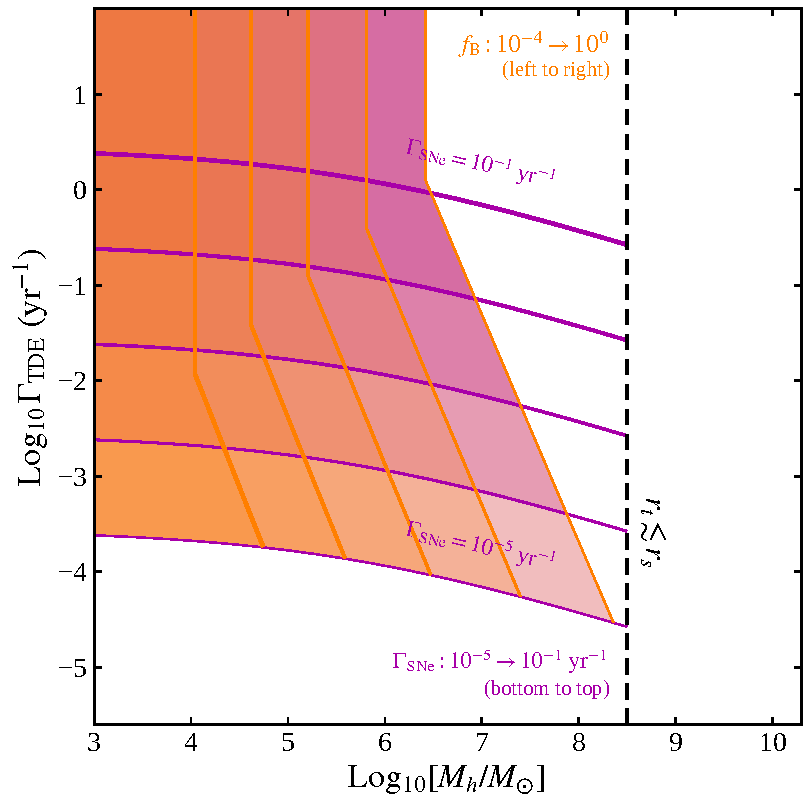
\includegraphics[width=0.9\linewidth,clip=true]{mom-rates.pdf}
\caption{Conditions by which TDEs dominate nuclear feedback for a variety of Bondi accretion efficiencies/Eddington ratios $f_{\rm Edd}^{2}/f_{\rm B}$ and local SNe rates $\Gamma_{\rm SNe}$, with $f_{\rm Edd}^{2}/f_{\rm B}$ varying from $10^{-4}$ to 1 from top to bottom and $\Gamma_{\rm SNe}$ varying from $10^{-5}$~yr$^{-1}$ to 0.1~yr$^{-1}$ from bottom to top (both in decade increments). Within the orange (purple) regions, TDEs dominate AGN (SNe) feedback for the given values of $f_{\rm Edd}^{2}/f_{\rm B}$ and $\Gamma_{\rm SNe}$. The vertical black dashed line indicates the limit where solar-mass stars are swallowed whole for non-spinning black holes before losing any mass via tides.}
\label{fig:rates}
\end{figure}

Comparing the most dominant subprocesses of Sections \ref{subsec:sne}, \ref{subsec:agn}, and \ref{subsec:tde} shows that if the tidal disruption rate is large, the momentum that TDEs provide can dominate all other forms of feedback, with the UDRs resulting from the unbound ejecta being the most important mechanism amongst the disruption feedback processes. By fixing the supernova rate and AGN accretion rates to fixed values, Figure \ref{fig:rates} shows the combinations of parameters for which tidal disruptions become the primary source of feedback for the MCs surrounding a SMBH of various masses. The figure shows that for a disruption rate $\Gamma_{\rm TDE} \sim 10^{-2}$, tidal disruptions beat out both AGN and SNe feedback processes \DIFdelbegin \DIFdel{if }\DIFdelend \DIFaddbegin \DIFadd{provided }\DIFaddend the AGN is only modestly active \DIFdelbegin \DIFdel{, $f_{\rm Edd}^{2}/f_{\rm B}~\sim~10^{-3}$, and if }\DIFdelend \DIFaddbegin \DIFadd{and }\DIFaddend the SNe rate does not exceed a value comparable to the rate within the MW's central kpc, $\Gamma_{\rm SNe} \sim 10^{-4}~{\rm yr}^{-1}$ (see Equation (\ref{eq:gammasne})).

\subsection{The collapse of externally-driven MCs and the underlying nucleus}

Assuming now that TDEs are primarily responsible for driving turbulence in the MCs surrounding the nucleus, the clouds will collapse gravitationally until they are in a new equilibrium where their enhanced level of turbulent support balances with their self-gravity. Because of the negative specific heat of self-gravitating systems \citep{Lynden-Bell:1968a}, the kinetic ``heating'' causes the density of the clouds to increase significantly (Figure \ref{fig:diagram}). Now denser, the MCs are free to dive deeper into the nuclear stellar cluster via dynamical friction without risk of tidal disruption by the black hole's gravity.

As the MCs burrow into the nucleus' outer layers, they proceed to scatter stars near them. This process removes the stars of lower binding energy, with the black hole only being able to retain the more-tightly bound stars closer to it. In an equilibrium state, the nuclear cluster surrounding the SMBH should have a mass of stars comparable to the mass of the SMBH. Restoring this equilibrium requires the black hole to capture stars of higher orbital energy that will not be removed by the MCs scouring its outer layers. Again, the negative specific heat of the system comes into play: In response to the frictive heating provided by the infalling MCs, the entire nucleus {\it also shrinks} until a new equilibrium is established\DIFdelbegin \DIFdel{where the denser MCs sit just outside of }\DIFdelend \DIFaddbegin \DIFadd{. As we show in Section~\ref{sec:equil}, the clouds do not come to rest at the sphere of influence itself, but settle at a radius roughly two orders of magnitude larger, where they can survive }\DIFaddend the black hole's \DIFdelbegin \DIFdel{new, smaller sphere of influence}\DIFdelend \DIFaddbegin \DIFadd{tidal field while still dominating the relaxation of the nucleus}\DIFaddend .

This effect is visible in N-body simulations of \citet{Antonini:2012a} (see their Figure 13) in which a massive body plunges into a SMBH cluster; the cluster shrinks in response to the presence of the sinking body. In the scenario proposed here, dozens of massive MCs drag into the nuclear cluster simultaneously, the cumulative effect of which enhances the cluster density to a value comparable to the density of the infalling MCs.

\subsection{An increased rate of disruptions and collisions}\label{subsec:increase}

With a higher stellar density and higher velocity dispersion, the two-body relaxation rate of the nuclear cluster shrinks dramatically, driving more stars into the loss cone and increasing the tidal disruption rate. These new disruptions further increase the rate of turbulent driving into the surrounding MCs, increasing their density, and thus further enhancing the rate. Without another process to halt the runaway, the stellar disruption rate could in principle become infinitely large.

Because the interactions between stars increases significantly, the rate of star-star collisions also increases as the nuclear cluster collapses. As we shall see in Section \ref{sec:collcond}, the rate of star-star collisions depends on the stellar density $n_{\ast}$, but the rate of tidal disruptions depends on the properties of the surrounding dense MCs. As a result, the rate of stellar collisions increases more rapidly than the rate of tidal disruptions, and at some point the probability that a star strikes another star becomes comparable to the rate it will be disrupted by the central black hole. 

As the stellar densities are largest closest to the black hole, most of the collisions occur just outside the tidal radius, the distance within which no stars exist. A star on its way to disruption would likely be scattered there in a single orbit about a normal nuclear cluster, but the compression of the core above the usual values means that even main-sequence stars are likely to be in the diffusion regime of disruption \citep{Wang:2004a,MacLeod:2012a}. In the diffusion regime, the stars spend many orbital periods in an orbit similar to their eventual disruptive orbit; each of these orbits presents the possibility of a stellar collision.

A collision between two stars effectively randomizes the orbits of the two stars (if they remain separate) or their merger product, removing them from the loss cone, and saving the star from being disrupted by the SMBH. This effectively caps the tidal disruption rate to a value no greater than the probability of stellar collision.

\section{Equilibrium state of TDE engines}\label{sec:equil}

A steady-state disruption engine requires the process to have both positive and negative feedback loops; if the disruption rate increases above its equilibrium value, some other process should act to reduce it back to this value, and vice versa if the disruption rate drops below this value. As discussed in the previous sections, disruptions enhance the nuclear density leading to more disruptions (the positive side of the loop), whereas collisions will prevent disruptions from exceeding a critical value (the negative side of the loop).

\DIFdelbegin \DIFdel{Although external pressure plays an important role in setting the volume of each cloud (and therefore the density), the external pressure equilibrium cannot prevent the clouds from being sheared away by the differential tidal force, which will eventually lead to individual clouds mixing with the ambient medium. Therefore, the critical criterion for a cloud's long-term survival is that it lies outside the tidal disruption radius, which is where the cloud's density is greater than the average density of the nuclear cluster $\rho_{\rm nc}$.
This sets the condition that
}\begin{displaymath}
\DIFdel{\rho_{\rm MC} = \rho_{\rm nc} \equiv \frac{9 M_{\rm h}}{4 \pi a_{\rm h}^{3}}
}\end{displaymath}%DIFAUXCMD
\DIFdel{In general, $a_{\rm h}$ is not known apriori as it is dependent on the stellar velocity dispersion }\DIFdelend \DIFaddbegin \subsection{\DIFadd{Structure of the nucleus and the surrounding cloud belt}}\label{subsec:structure}

\DIFadd{We describe the equilibrium with four quantities: the velocity dispersion }\DIFaddend $\sigma$ \DIFdelbegin \DIFdel{just outside the }\DIFdelend \DIFaddbegin \DIFadd{that sets the size of the sphere of influence, the radius $r_{\rm b}$ at which the molecular clouds orbit, their internal Mach number ${\cal M}$, and their radius $R_{\rm MC}$. Three physical conditions, described in the following section, close the system, leaving $M_{\rm h}$ (and the Bondi efficiency $f_{\rm B}$, which enters only the derived accretion quantities) as the sole free parameter.
}

\DIFadd{The stellar cluster is taken to be a relaxed Bahcall-Wolf cusp, $n_{\ast}(r) \propto r^{-\gamma}$ with $\gamma = 7/4$, containing a mass in stars equal to twice the black hole mass within its }\DIFaddend sphere of influence,
\begin{equation}
a_{\rm h} = \DIFdelbegin \DIFdel{\frac{G M_{\rm h}}{\sigma^{2}} }\DIFdelend \DIFaddbegin \DIFadd{\frac{2 G M_{\rm h}}{\sigma^{2}} }\DIFaddend = 1.5 \mhsix \sigma_{75}^{-2}~{\rm pc},\DIFaddbegin \label{eq:ah}
\DIFaddend \end{equation}
where $\sigma_{75}$ is $\sigma$ in units of $75~{\rm km~s}^{-1}$. \DIFdelbegin \DIFdel{Because the density of MCs and the nuclear cluster are equal, we can calculate density of both by determining the density of the MCs.
The ambient pressure of the gas surrounding the MCs, assuming that the hot phase gas is virialized with $k T = m_{\rm p} \sigma^{2} / k_{\rm b}$, is equal to }\DIFdelend \DIFaddbegin \DIFadd{With an average stellar mass $m_{\ast} = 0.5~\msun$ and radius $R_{\ast} = 0.46~R_{\odot}$ \mbox{%DIFAUXCMD
\citep{Tout:1996a}}\hskip0pt%DIFAUXCMD
, the number of stars is $N_{\ast} = 2 M_{\rm h}/m_{\ast}$ and the density normalization of }\DIFaddend the \DIFdelbegin \DIFdel{turbulent pressure holding up the cloudagainst gravity. We define the turbulent velocity within the cloud $\sigma_{\rm cloud}$ in terms of the Mach number and the sound speed, $\sigma_{\rm cloud} = {\cal M}_{\rm MC} c_{\rm s}$, with $c_{\rm s} = \sqrt{5 k_{\rm b} T_{\rm cl} / 3 \mu m_{\rm p}}$. If we presume that the clouds are self-gravitating, the free-fall time will be defined by the turbulent velocity within the cloud, and will be equal to the free-fall time of the nuclear cluster by definition as they are placed at their disruption radius. As the crossing time $\tau_{\rm c} = 3 \tau_{\rm ff} / {\cal M}_{\rm MC}$,
we find
}\DIFdelend \DIFaddbegin \DIFadd{cusp is $n_{0} = (3-\gamma)N_{\ast}/4\pi a_{\rm h}^{3}$. Within the cusp the one-dimensional dispersion is $\sigma_{\rm h} = \sigma/\sqrt{2}$.
}

\DIFadd{The molecular clouds cannot themselves reside at $a_{\rm h}$. This is a departure from the picture sketched in Section~\ref{sec:engine}, and it is forced on us by the solution: at the compressed densities the cluster reaches, a cloud placed at $a_{\rm h}$ would need a density $\gtrsim 10^{10}~{\rm cm}^{-3}$ to survive the black hole's tidal field, at which point no UDR could drive it (its radiative length would fall below the cloud's own size), and the first of our conditions below has no solution. The clouds instead settle into a belt at a radius $r_{\rm b} \gg a_{\rm h}$, where the tidal limit is far less severe. Structures of exactly this kind are now routinely resolved: ALMA imaging of NGC~1068 reveals a rotating molecular disk of $\sim 10^{5}~\msun$ and $7$--$10$~pc diameter surrounding the black hole \mbox{%DIFAUXCMD
\citep{GarciaBurillo:2016a,Imanishi:2018a,Impellizzeri:2019a}}\hskip0pt%DIFAUXCMD
, and surveys of nearby Seyferts find such compact molecular disks to be the norm rather than the exception, with median diameters of tens of parsecs and masses of a few $\times 10^{5}~\msun$ \mbox{%DIFAUXCMD
\citep{Combes:2019a,GarciaBurillo:2021a}}\hskip0pt%DIFAUXCMD
. Our own Galactic center hosts the same structure at smaller scale in its circumnuclear disk. The radius and mass we derive below are set by the equilibrium conditions rather than fitted, and it is worth stating in advance that they land close to these observed values. There they are marginally tidally bound,
}\DIFaddend \begin{equation}
\DIFdelbegin \DIFdel{\tau_{\rm c} }\DIFdelend \DIFaddbegin \DIFadd{\rho_{\rm MC} }\DIFaddend = \DIFdelbegin \DIFdel{\frac{3 \pi}{{\cal M}_{\rm MC}} }%DIFDELCMD < \left(%%%
\DIFdel{\frac{a_{\rm h}^{3}}{G M_{\rm h}}}%DIFDELCMD < \right)%%%
\DIFdel{^{1/2}.
}\DIFdelend \DIFaddbegin \DIFadd{\frac{9 M_{\rm h}}{4 \pi r_{\rm b}^{3}},}\label{eq:rhomc}
\DIFaddend \end{equation}
\DIFdelbegin \DIFdel{Finally, the density of the cloud can be determined from the crossing time
}\begin{displaymath}
\DIFdel{\rho_{\rm MC} = \frac{0.54}{G \tau_{\rm c}^{2}},
}\end{displaymath}%DIFAUXCMD
\DIFdel{which can be rewritten in terms of $\sigma$ and ${\cal M}_{\rm MC}$,
}\begin{align*}
\DIFdel{\rho_{\rm MC} }&\DIFdel{= 1 \times 10^{-18} \mhsix^{-2} \left(\frac{{\cal M}_{\rm MC}}{3}\right)^{2} \sigma_{75}^{6}.
}\end{align*}%DIFAUXCMD
%DIFDELCMD < 

%DIFDELCMD < %%%
\DIFdel{There are of course need to be many MCs surrounding the black hole to cover the full $4\pi$ steradians of solid angle. If each cloud has a radius $R_{\rm MC}$ and mass $M_{\rm MC}$, the total mass is divided into a finite number of clouds $N_{\rm MC}$. Given $\rho_{\rm MC}$ }\DIFdelend and \DIFdelbegin \DIFdel{$R_{\rm MC}$, the number of clouds is }\begin{displaymath}
\DIFdel{N_{\rm MC} = \frac{4 a_{\rm h}^{2}}{R_{\rm MC}^{2}}
}\end{displaymath}%DIFAUXCMD
\DIFdelend \DIFaddbegin \DIFadd{supported against their own self-gravity by supersonic turbulence,
}\begin{equation}
{\DIFadd{\cal M}}\DIFadd{^{2} c_{\rm s}^{2} = \frac{4 \pi}{5} G \rho_{\rm MC} R_{\rm MC}^{2},\label{eq:virial}
}\end{equation}\DIFaddend 
\DIFdelbegin \DIFdel{and }\DIFdelend \DIFaddbegin \DIFadd{with $c_{\rm s} = 0.19~{\rm km~s}^{-1}$ the isothermal sound speed of $10$~K molecular gas at $\mu = 2.33$. The turbulent velocity within each cloud is $\sigma_{\rm cl} = {\cal M} c_{\rm s}$ and the crossing time on which that turbulence decays is $\tau_{\rm c} = 2 R_{\rm MC}/\sigma_{\rm cl}$. The number density of gas in a cloud is $n_{\rm MC} = \rho_{\rm MC}/1.4 m_{\rm p}$, the }\DIFaddend mass of each cloud is \DIFdelbegin \begin{displaymath}
\DIFdel{M_{\rm MC} = \frac{4\pi}{3} \rho_{\rm MC} R_{\rm MC}^{3}.
}\end{displaymath}%DIFAUXCMD
\DIFdelend \DIFaddbegin \DIFadd{$M_{\rm MC} = 4 \pi \rho_{\rm MC} R_{\rm MC}^{3}/3$, and $N_{\rm MC} = 4 r_{\rm b}^{2}/R_{\rm MC}^{2}$ clouds are required to cover the belt.
}\DIFaddend 

\DIFaddbegin \DIFadd{That the clouds sit well outside the cusp is what allows them to keep the loss cone full while remaining dynamically benign for the cusp itself, as we discuss in Section~\ref{sec:collcond}.
}

\DIFaddend \subsection{Conditions for equilibrium}\DIFaddbegin \label{subsec:conditions}
\DIFaddend 

\DIFdelbegin \DIFdel{To determine an equilibrium for a given black hole mass $M_{\rm h}$, we solve a system of three algebraic expressions that relate the velocity dispersion $\sigma$, Mach number $\mathcal{M}$, and radii of the MCs $R_{\rm MC}$. These expressions are related to the finite sizes of the UDRs, the heating and cooling of the MCs, and the condition that the rate of star-star collisions equals the rate of disruptions.
The three expressions are summarized below.
}%DIFDELCMD < 

%DIFDELCMD < %%%
%DIF < $\mu = 0.5$, the cloud mass ratio relative to the black hole mass ${\cal Q}_{\rm cl} \equiv M_{\rm cl} / M_{\rm h}$, ambient medium virial temperature $T_{\rm bg} = m_{\rm p} \sigma^{2} / 3 k_{\rm b}$, where $\sigma$ is the Keplerian velocity dispersion, $T_{\rm cl}$ the molecular clouds' gas temperature. The clouds are supported against the ambient pressure and self-gravity by supersonic turbulence with 
%DIFDELCMD < 

%DIFDELCMD < %%%
\DIFdelend \subsubsection{Finite sizes of UDRs}

While more momentum can be driven into the MCs by the UDRs than any other process, it is not necessarily the case that this momentum will be shared equally amongst all MCs surrounding the SMBH. Each UDR will only be in contact with a size scale comparable to its Sedov-Taylor length $R_{\rm ST}$, which \DIFdelbegin \DIFdel{can be somewhat smaller than the black hole's sphere of influence}\DIFdelend \DIFaddbegin \DIFadd{is small compared to the belt radius}\DIFaddend . As all MCs must be struck at least once per crossing time to sustain their turbulent energy, multiple tidal disruptions are required to cover the full $4\pi$ steradians of solid angle surrounding the black hole\DIFdelbegin \DIFdel{to ensure that all MCs in the vicinity of the nucleus are driven by TDE feedback}\DIFdelend . This sets our first condition,
\begin{equation}
\Gamma_{\rm TDE} f_{\rm UDR} \DIFdelbegin \DIFdel{= }\DIFdelend \tau_{\rm c} \DIFdelbegin \DIFdel{^{-1}}\DIFdelend \DIFaddbegin \DIFadd{= 1}\DIFaddend ,\label{eq:cond1}
\end{equation}
where \DIFdelbegin \DIFdel{$f_{\rm UDR}$ }\DIFdelend \DIFaddbegin \DIFadd{$f_{\rm UDR} = R_{\rm UDR}^{2}/4 r_{\rm b}^{2}$ }\DIFaddend is the fractional solid angle occupied by a single UDR. %DIF < For clouds in our own galactic center, the typical densities of the non-star-forming clouds is $10^{4}$~cm$^{-3}$, with Mach numbers ${\cal M}$ of a few being typical \colr{citation}.
\DIFdelbegin \DIFdel{This fraction is }\DIFdelend \DIFaddbegin \DIFadd{This fraction }\DIFaddend depends on the Sedov-Taylor length \citep{Sedov:1946a,Taylor:1950a} within the clouds the UDRs are striking,
\begin{equation}
R_{\rm ST} = 1.15 \left(\frac{E}{\rho_{\rm MC}}\right)^{1/5} \tau_{\rm rad}^{2/5}\DIFdelbegin %DIFDELCMD < \label{eq:rst}%%%
\DIFdelend ,\DIFaddbegin \label{eq:rst}
\DIFaddend \end{equation}
where $\tau_{\rm rad}$ is the timescale for the UDR to become radiative\DIFdelbegin \DIFdel{. $\tau_{\rm rad}$ is }\DIFdelend \DIFaddbegin \DIFadd{, itself }\DIFaddend set by the density of the clouds being impacted,
\begin{equation}
\tau_{\rm rad} = 130 E_{50}^{4/17}n_{\rm MC,4}^{-9/17}~{\rm yr}\DIFdelbegin \DIFdel{.}\DIFdelend \DIFaddbegin \DIFadd{,}\DIFaddend \label{eq:trad}
\end{equation}
\DIFaddbegin \DIFadd{following the numerical SNR calculations of \mbox{%DIFAUXCMD
\citet{Blondin:1998a}}\hskip0pt%DIFAUXCMD
. }\DIFaddend Assuming a solar composition and combining Equations (\ref{eq:rst}) and (\ref{eq:trad}), we find
\begin{equation}
R_{\rm UDR} = \DIFdelbegin \DIFdel{0.24 }\DIFdelend \DIFaddbegin \DIFadd{0.22 }\DIFaddend E_{50}^{5/17} n_{\rm MC,4}\DIFdelbegin \DIFdel{^{-18/85}}\DIFdelend \DIFaddbegin \DIFadd{^{-7/17}}\DIFaddend ~{\rm pc}\DIFdelbegin \DIFdel{.
}\DIFdelend \DIFaddbegin \DIFadd{,}\label{eq:rudr}
\DIFaddend \end{equation}
\DIFaddbegin \DIFadd{evaluated at the cloud density $n_{\rm MC}$. }\DIFaddend At this distance \DIFdelbegin \DIFdel{, }\DIFdelend the remnant begins to radiate away much of its energy rather than depositing it into the surrounding MCs, and it is at this time that the majority of the momentum is deposited as the remnant sweeps up a mass several times its own. Note that these expressions presume the UDR solely interacts with the cold MC gas phase and not the surrounding hot phase; because of its much lower density, a UDR will propagate to a much larger size before becoming radiative in the hot phase. However, the unbound debris streams that produce UDRs will almost certainly strike a dense MC before reaching their termination distance in the surrounding hot ISM \citep{Guillochon:2016b}, with the MCs having a solid angle coverage fraction of order unity even in our own MW \citep{Chen:2016b}, which is a tepid accretor.

\DIFdelbegin \DIFdel{If we assume an unbound stream halts its outward progress at $r = a_{\rm h}$ where the MCs begin to exist, it will affect a fractional solid angle of MCs equal to $R_{\rm UDR}^{2}/4 a_{\rm h}^{2}$,
}\begin{align*}
\DIFdel{f_{\rm UDR} }&\DIFdel{= 6 \times 10^{-3} E_{50}^{5/17} n_{\rm MC,4}^{-18/85} \mhsix^{-2}\sigma_{75}^{4}.
}\end{align*}%DIFAUXCMD
%DIFDELCMD < 

%DIFDELCMD < %%%
\DIFdelend \subsubsection{Heating and cooling of MCs}

Both momentum and energy are injected into the MCs as UDRs slam into them. As turbulence decays, the kinetic energy of the turbulence is converted into heat, which the cloud must radiate away at \DIFdelbegin \DIFdel{a rate that is faster than the rate of energy injection}\DIFdelend \DIFaddbegin \DIFadd{the same rate at which energy is being injected}\DIFaddend . This defines a second condition,
\begin{equation}
\DIFdelbegin \DIFdel{L_{\rm MC} }\DIFdelend \DIFaddbegin \DIFadd{\Gamma_{\rm TDE} E_{\rm UDR} }\DIFaddend = L\DIFdelbegin \DIFdel{_{\rm UDR}}\DIFdelend \DIFaddbegin \DIFadd{_{\rm MC}}\DIFaddend ,\label{eq:cond2}
\end{equation}
where \DIFaddbegin \DIFadd{$E_{\rm UDR} = 1.8 \times 10^{50} \mhsix^{1/3}$~ergs is the energy of the unbound debris \mbox{%DIFAUXCMD
\citep{Guillochon:2016b} }\hskip0pt%DIFAUXCMD
and }\DIFaddend $L_{\rm MC}$ is the total cooling rate of all MCs \DIFdelbegin \DIFdel{surrounding the nuclear cluster}\DIFdelend \DIFaddbegin \DIFadd{in the belt}\DIFaddend . Because the rate of cooling is a steep function of temperature below H-recombination, the MCs rapidly cool to a temperature where their cooling rates are equal to the cosmic ray heating rate, $\sim 10~{\rm K}$ \citep{Krumholz:2015a}, with CO cooling being the predominant coolant. \DIFdelbegin \DIFdel{Thus, the total cooling rate is equal to the CO cooling rate multiplied by the total volume of the MCs,
}\begin{align*}
\DIFdel{L_{\rm MC} = \Lambda_{\rm CO} N_{\rm MC} V_{\rm MC},
}\end{align*}%DIFAUXCMD
\DIFdelend \DIFaddbegin \DIFadd{Writing the volumetric cooling rate as $\Lambda_{0} n_{\rm MC}^{2}$ with $\Lambda_{0} = 1.3 \times 10^{-27}~{\rm erg~cm}^{3}~{\rm s}^{-1}$ \mbox{%DIFAUXCMD
\citep{Goldsmith:1978a,Neufeld:1995a,Goldsmith:2001a}}\hskip0pt%DIFAUXCMD
, and summing over the $N_{\rm MC}$ clouds of the belt,
}\begin{equation}
\DIFadd{L_{\rm MC} = \frac{16 \pi}{3} \Lambda_{0} n_{\rm MC}^{2} r_{\rm b}^{2} R_{\rm MC}.\label{eq:lmc}
}\end{equation}\DIFaddend 
\DIFdelbegin \DIFdel{where $V_{\rm MC} \equiv 4 \pi \rho_{\rm MC} R_{\rm MC}^{3}/3$ is the volume of each cloud.
}\DIFdelend 

\subsubsection{Stellar collisions preventing a disruption runaway}\label{sec:collcond}

As described in Section \ref{subsec:increase}, the rate of star-star collisions in an isotropic cluster increases as the density of the cluster increases during the collapse of the nuclear cluster. For a star to be successfully disrupted, it must run the gauntlet of the high-density central region of the cluster where it is at risk of colliding with another star. This yields our last condition,
\begin{equation}
\DIFdelbegin \DIFdel{\gamma_{\rm TDE}(r_{\rm i}) = \gamma}\DIFdelend \DIFaddbegin \DIFadd{\Gamma}\DIFaddend _{\rm coll} \DIFdelbegin \DIFdel{(r_{\rm i}),}\DIFdelend \DIFaddbegin \DIFadd{= \Gamma_{\rm TDE}.}\DIFaddend \label{eq:cond3}
\end{equation}
\DIFaddbegin \DIFadd{The two rates on either side of this expression must be evaluated with some care, and both differ from the estimates used in earlier treatments of this problem.
}

\DIFadd{Because the stellar density rises steeply toward the center, we obtain $\Gamma_{\rm coll}$ by integrating the collision rate over the cusp rather than evaluating it at a single radius. Crucially, at the densities of interest the orbital speeds within most of the cusp remain below the escape speed from a star's own surface, $v_{\rm esc,\ast} = 644~{\rm km~s}^{-1}$, so collisions are gravitationally focused and the geometric cross-section badly underestimates the rate. Retaining the focusing term, integration of $n_{\ast}^{2} \Sigma_{\rm coll} v$ over the $\gamma = 7/4$ cusp gives
}\begin{equation}
\DIFadd{\Gamma_{\rm coll} = 8 \pi^{2} \Lambda_{\rm c} R_{\ast}^{2} v_{\rm esc,\ast}^{2} n_{0}^{2} a_{\rm h}^{7/2} \left(G M_{\rm h}\right)^{-1/2},\label{eq:gcoll}
}\end{equation}
\DIFadd{where $\Lambda_{\rm c} \simeq 3$ collects the dimensionless integral over the cusp profile. Neglecting focusing, as is sometimes done, moves the collisional cap to velocity dispersions that are not physically attainable.
}

\DIFadd{For the disruption rate we take the full-loss-cone (pinhole) rate, appropriate when the angular momentum a star receives per orbit exceeds the width of the loss cone. Massive perturbers keep the loss cone full in exactly this way \mbox{%DIFAUXCMD
\citep{Perets:2007a}}\hskip0pt%DIFAUXCMD
, and the belt clouds derived above are massive perturbers of the required magnitude. Following \mbox{%DIFAUXCMD
\citet{Syer:1999a} }\hskip0pt%DIFAUXCMD
and \mbox{%DIFAUXCMD
\citet{Stone:2016a}}\hskip0pt%DIFAUXCMD
,
}\begin{equation}
\DIFadd{\Gamma_{\rm TDE} = 4 \times 10^{-5} \mhsix^{4/3}\left(\frac{n_{0}}{10^{5}~{\rm pc}^{-3}}\right)\left(\frac{100~{\rm km~s}^{-1}}{\sigma_{\rm h}}\right)^{3}~}{\DIFadd{\rm yr}}\DIFadd{^{-1},\label{eq:gtde}
}\end{equation}
\DIFadd{which is equivalent to $\Gamma_{\rm TDE} \propto n_{0} r_{\rm t} G M_{\rm h}/\sigma_{\rm h}$ up to the numerical prefactor.
}

\DIFadd{Equations~(\ref{eq:gcoll}) and (\ref{eq:gtde}) both depend only on $\sigma$ once $M_{\rm h}$ is fixed, so Equation~(\ref{eq:cond3}) alone determines the compression of the cluster; the remaining two conditions then fix the properties of the belt.
}

\subsection{\DIFadd{The Engine State}}\label{subsec:engine-state}

\DIFadd{The three conditions (Equations (\ref{eq:cond1}), (\ref{eq:cond2}), and (\ref{eq:cond3})) are each monomial in the four unknowns, and so the system can be solved in closed form by taking logarithms; the solution is a set of exact power laws in $M_{\rm h}$, which we quote below to two significant figures. For the nuclear cluster we find
}\begin{align}
\DIFadd{\sigma }&\DIFadd{= 4.0 \times 10^{2} \mhsix^{1/6}~}{\DIFadd{\rm km~s}}\DIFadd{^{-1}}\\
\DIFadd{a_{\rm h} }&\DIFadd{= 5.5 \times 10^{-2} \mhsix^{2/3}~}{\DIFadd{\rm pc}}\\
\DIFadd{n_{0} }&\DIFadd{= 2.4 \times 10^{9} \mhsix^{-1}~}{\DIFadd{\rm pc}}\DIFadd{^{-3}}\\
\DIFadd{P_{\rm h} }&\DIFadd{= 1.2 \times 10^{3} \mhsix^{1/2}~}{\DIFadd{\rm yr}}\\
\DIFadd{\tau_{\rm relax,\ast} }&\DIFadd{= 1.9 \times 10^{8} \mhsix^{3/2}~}{\DIFadd{\rm yr}}\DIFadd{,
}\end{align}
\DIFaddend where \DIFdelbegin \DIFdel{$\gamma_{\rm TDE}(r_{\rm i})$ }\DIFdelend \DIFaddbegin \DIFadd{$P_{\rm h}$ is the orbital period at $a_{\rm h}$ }\DIFaddend and \DIFdelbegin \DIFdel{$\gamma_{\rm coll}(r_{\rm i})$ are the specific rates of disruption and collision for a single star with periapse $r_{\rm p} = r_{\rm i}$, where $r_{\rm i}$ is }\DIFdelend \DIFaddbegin \DIFadd{$\tau_{\rm relax,\ast}$ }\DIFaddend the \DIFdelbegin \DIFdel{innermost radius for which stars exist.
Depending on which process dominates for star loss (disruptions or collisions) , $r_{\rm i}$ could be equal to $r_{\rm t}$, or it could be equal to $r_{\rm c}$, the distance within which the depletion by stars via collisions is comparable to the }\DIFdelend \DIFaddbegin \DIFadd{two-body }\DIFaddend relaxation time of the \DIFdelbegin \DIFdel{cluster. }%DIFDELCMD < 

%DIFDELCMD < %%%
\DIFdel{Because of the steep density gradient of stars in a nuclear cluster, the majority of collisions take place at its center, and thus the total collision rate of the cluster $\Gamma_{\rm coll}$ can be approximated by calculating the collision rate at that location. As $r_{\rm i}$ is the minimum distance stars can exist, this means the rate of collisions is
}\DIFdelend \DIFaddbegin \DIFadd{cusp. The properties of the belt and of the clouds within it are
}\begin{align}
\DIFadd{r_{\rm b} }&\DIFadd{= 6.4 \mhsix^{0.66}~}{\DIFadd{\rm pc}}\\
{\DIFadd{\cal M}} &\DIFadd{= 37 \mhsix^{0.31}}\\
\DIFadd{R_{\rm MC} }&\DIFadd{= 1.3 \mhsix^{0.79}~}{\DIFadd{\rm pc}}\\
\DIFadd{n_{\rm MC} }&\DIFadd{= 8.0 \times 10^{4} \mhsix^{-0.97}~}{\DIFadd{\rm cm}}\DIFadd{^{-3}}\\
\DIFadd{\sigma_{\rm cl} }&\DIFadd{= 6.9 \mhsix^{0.31}~}{\DIFadd{\rm km~s}}\DIFadd{^{-1}}\\
\DIFadd{\tau_{\rm c} }&\DIFadd{= 3.6 \times 10^{5} \mhsix^{0.49}~}{\DIFadd{\rm yr}}\\
\DIFadd{M_{\rm MC} }&\DIFadd{= 2.3 \times 10^{4} \mhsix^{1.41}~\msun}\\
\DIFadd{N_{\rm MC} }&\DIFadd{= 1.0 \times 10^{2} \mhsix^{-0.27}}\\
\DIFadd{M_{\rm belt} }&\DIFadd{= 2.4 \times 10^{6} \mhsix^{1.14}~\msun,
}\end{align}
\DIFadd{corresponding to a gas surface density through the belt of $1.9 \times 10^{4}~\msun~{\rm pc}^{-2}$. The equilibrium disruption rate is
}\begin{equation}
\DIFadd{\Gamma_{\rm eq} = \Gamma_{\rm coll} = 3.7 \times 10^{-2} \mhsix^{-1/6}~}{\DIFadd{\rm yr}}\DIFadd{^{-1},\label{eq:eqrate}
}\end{equation}
\DIFadd{a factor of several hundred above the canonical $10^{-4}$~yr$^{-1}$, and with only a very weak (and now inverted) dependence on black hole mass. The size, radiative time, angular coverage, and collective luminosity of the UDRs are
}\begin{align}
\DIFadd{R_{\rm UDR} }&\DIFadd{= 0.11 \mhsix^{1/2}~}{\DIFadd{\rm pc}}\\
\DIFadd{\tau_{\rm rad} }&\DIFadd{= 49 \mhsix^{0.59}~}{\DIFadd{\rm yr}}\\
\DIFadd{f_{\rm UDR} }&\DIFadd{= 7.6 \times 10^{-5} \mhsix^{-0.32}}\\
\DIFadd{L_{\rm UDR} = L_{\rm MC} }&\DIFadd{= 2.1 \times 10^{41} \mhsix^{1/6}~}{\DIFadd{\rm erg~s}}\DIFadd{^{-1}.
}\end{align}
\DIFadd{The density of the gas surrounding the black hole, the resulting accretion luminosity, and the typical extinction through the ambient medium are
}\begin{align}
\DIFadd{n_{\rm bg} }&\DIFadd{= 5.7 \times 10^{3} \mhsix^{-0.70}~}{\DIFadd{\rm cm}}\DIFadd{^{-3}}\\
\DIFadd{L_{\rm AGN}/L_{\rm Edd} }&\DIFadd{= 6.0 \times 10^{-2} f_{\rm B,-3} \mhsix^{-0.21}}\\
\DIFadd{A_{\rm V} }&\DIFadd{\simeq 51 \mhsix^{-0.04},
}\end{align}
\DIFadd{and finally the average feeding rate of the black hole from TDEs relative to accretion of the surrounding gas is
}\DIFaddend \begin{equation}
\DIFdelbegin \DIFdel{\Gamma_{\rm coll} = N_{\rm i}^{2}\sigma_{\ast}v_{\rm i}}\DIFdelend \DIFaddbegin \langle \dot{M}\DIFadd{_{\rm TDE} }\rangle \DIFaddend / \DIFdelbegin \DIFdel{V_{\rm i}
}\DIFdelend \DIFaddbegin \dot{M}\DIFadd{_{\rm amb} = 3.5 f_{\rm B,-3}^{-1}}\mhsix\DIFadd{^{-0.96}.}\label{eq:eqaccratio}
\DIFaddend \end{equation}
\DIFdelbegin \DIFdel{where $N_{\rm i} = n_{\rm i} V_{\rm i}$ is the total number of stars contained in this region $V_{\rm i} = 4 \pi n_{\ast} r_{i}^{3}/3$ is the volume of the region, $\sigma_{\ast} \equiv \pi R_{\ast}^{2}$ is the physical cross-section of each star (at these distances, the orbital velocity is much larger than the stellar escape velocity and gravitational focusing can be ignored), }\DIFdelend \DIFaddbegin 

\DIFadd{Several features of this solution deserve comment. The equilibrium is remarkably insensitive to black hole mass: $\Gamma_{\rm eq}$ varies by only a factor of three across the four decades of $M_{\rm h}$ over which the engine can operate. The clouds that emerge are not exotic. With $n_{\rm MC} \sim 10^{5}~{\rm cm}^{-3}$, $\sigma_{\rm cl} \sim 7~{\rm km~s}^{-1}$, radii of order a parsec, and strongly suppressed star formation, they are close analogues of the clouds observed in the Milky Way's own Central Molecular Zone, of which G0.253+0.016 (``the Brick'') is the best-studied example \mbox{%DIFAUXCMD
\citep{Longmore:2013a,Kruijssen:2014a,Barnes:2017a}}\hskip0pt%DIFAUXCMD
. The engine state, in other words, does not require gas in an unobserved configuration; it requires CMZ-like gas around a nucleus in which the disruption rate has already been raised.
}

\DIFadd{The extinction is the most immediately testable consequence: $A_{\rm V} \simeq 50$ means that an engine nucleus is optically obscured, and its disruptions would be missed entirely by optical surveys while remaining detectable in the infrared.
}

\DIFadd{We also note the assumptions that limit the range of validity of Equations (\ref{eq:eqrate})--(\ref{eq:eqaccratio}). The gravitational focusing that sets Equation~(\ref{eq:gcoll}) requires $\sigma_{\rm h} < v_{\rm esc,\ast}$, which fails for $M_{\rm h} \gtrsim 10^{8}~\msun$; above $10^{8.5}~\msun$ main-sequence stars are swallowed whole in any case. At the other end, the ratio of the per-orbit angular momentum kick to the loss cone width for cusp stars is $q_{\ast} = 0.14 \mhsix^{-2/3}$, placing the cusp near the boundary between the full and empty loss cone regimes rather than safely within the former. Equation~(\ref{eq:gtde}) is therefore an upper envelope on the disruption rate, }\DIFaddend and \DIFdelbegin \DIFdel{$v_{\rm i} = \sqrt{G M_{\rm h}/r_{\rm i}}$ is the typical velocity of }\DIFdelend \DIFaddbegin \DIFadd{$\Gamma_{\rm eq}$ should be read as such. We note that the belt clouds cannot themselves torque cusp stars efficiently ($q_{\rm MC} \sim 10^{-8}$ for a star deep in }\DIFaddend the \DIFdelbegin \DIFdel{stars at the tidal radius. }\DIFdelend \DIFaddbegin \DIFadd{cusp, though $q_{\rm MC} \gg 1$ at the belt radius itself); the loss cone is more plausibly kept populated by stars formed in the belt clouds on low-angular-momentum orbits, which is the resupply channel implied by the association of TDEs with recent star formation.
}\DIFaddend 

\DIFdelbegin \DIFdel{Our condition (Equation (\ref{eq:cond3})) implies that }%DIFDELCMD < {\it %%%
\DIFdel{the same stars that would be disrupted end up colliding with another star first}%DIFDELCMD < }%%%
\DIFdel{.
It is not enough then simply for the total rates of collisions and tidal disruptions in the entire cluster to be equal, the rates must be the same for the stars that will eventually be disrupted, these are stars that are near the loss cone in angular momentum space but not within it yet. }\DIFdelend \DIFaddbegin \subsection{\DIFadd{Disk geometry and the direction of the debris}}\label{subsec:disk}
\DIFaddend 

\DIFdelbegin \DIFdel{While more sophisticated approaches exist for calculating the tidal disruption rate\mbox{%DIFAUXCMD
\citep[see e.g.][]{Magorrian:1999a,Wang:2004a,Stone:2016a}}\hskip0pt%DIFAUXCMD
, the simplest is to note that a given star within a nuclear cluster will fully explore its available angular momentum and energy phase space in a relaxation time, which involves its eventual traversal of the loss-cone region. With $N$ stars total in the cluster, this yields an expression for the disruption rate of \mbox{%DIFAUXCMD
\citep{Lightman:1977a}}\hskip0pt%DIFAUXCMD
,
}\begin{displaymath}
\DIFdel{\Gamma_{\rm TDE} = N/\tau_{\rm relax},
}\end{displaymath}%DIFAUXCMD
\DIFdelend \DIFaddbegin \DIFadd{The solution above treats the clouds as a spherical belt covering $4\pi$ steradians. This is almost certainly wrong in detail. Gas that settles in a galactic nucleus carries angular momentum, and the structures actually resolved around nearby black holes are disks: the NGC~1068 torus is a rotating molecular disk a few parsecs across \mbox{%DIFAUXCMD
\citep{GarciaBurillo:2016a,Imanishi:2018a,Impellizzeri:2019a}}\hskip0pt%DIFAUXCMD
, and compact molecular disks of comparable size and mass are found in most nearby Seyferts surveyed \mbox{%DIFAUXCMD
\citep{Combes:2019a,GarciaBurillo:2021a}}\hskip0pt%DIFAUXCMD
. We therefore let the clouds occupy a disk of aspect ratio
}\begin{equation}
\DIFadd{f_{\Omega} \equiv H/r_{\rm b},
}\end{equation}\DIFaddend 
\DIFdelbegin \DIFdel{where the relaxation time $\tau_{\rm relax}$ is set by the dominant perturbers of the cluster, }\begin{displaymath}
\DIFdel{\tau_{\rm relax}^{-1} = \log \Lambda \frac{G^{2}}{\sigma^{3}} M^{2} n,
}\end{displaymath}%DIFAUXCMD
\DIFdel{where $\log \Lambda \sim 10$ is the standard Coulomb logarithm and $n$ is the number density of the perturbers. When the perturbers are the stars themselves, $n$ is the stellar number density, and the disruption rate would scale as the number of stars squared, just as the collision rate does. However, when the dominant perturbers are molecular clouds, $n \equiv N_{\rm mc} / V_{\rm cover}$, the number density of clouds in the nuclear clusters' vicinity, where $V_{\rm cover}\equiv f_{\rm vol} V_{\rm MC}$ is the total volume extending to the distance where the clouds would cover }\DIFdelend \DIFaddbegin \DIFadd{which is the fraction of }\DIFaddend $4\pi$ \DIFdelbegin \DIFdel{steradians. Given the volume of each cloud $V_{\rm MC}$ and the total number of clouds $N_{\rm MC}$, }\DIFdelend \DIFaddbegin \DIFadd{the disk subtends as seen from the black hole. Observed circumnuclear disks are geometrically thick, with $f_{\Omega} \sim 0.1$--$0.3$; we adopt $f_{\Omega} = 0.2$ as a fiducial value and quote the scalings explicitly.
}

\subsubsection{\DIFadd{Why the spherical solution survives an isotropic cusp}}

\DIFadd{It is worth noting first that if the stellar cusp remains isotropic, flattening the gas into a disk changes nothing at all; two factors of $f_{\Omega}$ enter and cancel: the number of clouds needed to cover }\DIFaddend the \DIFdelbegin \DIFdel{relaxation time when molecular clouds dominate the relaxation process is directly related to the clouds' densities, }\begin{displaymath}
\DIFdel{\tau_{\rm relax}^{-1} = \log \Lambda \frac{G^{2}}{\sigma^{3}} M_{\rm MC} \rho_{\rm MC}.%DIFDELCMD < \label{eq:trelmc}%%%
}\end{displaymath}%DIFAUXCMD
\DIFdelend \DIFaddbegin \DIFadd{structure drops to $N_{\rm MC} = 4 f_{\Omega} r_{\rm b}^{2}/R_{\rm MC}^{2}$, reducing the total cooling rate by $f_{\Omega}$; but only a fraction $f_{\Omega}$ of isotropically directed UDRs strike the disk at all, reducing the heating rate by the same factor. Condition (\ref{eq:cond2}) is therefore unchanged. The same cancellation occurs in condition (\ref{eq:cond1}): there is less sky to cover, but proportionally fewer remnants doing the covering, and the covering time $4 f_{\Omega} r_{\rm b}^{2}/(\Gamma f_{\Omega} R_{\rm UDR}^{2})$ is independent of $f_{\Omega}$.
}

\DIFadd{Every quantity in Section~\ref{subsec:engine-state} thus carries over unmodified, with the single exception of the total gas mass, which becomes
}\begin{equation}
\DIFadd{M_{\rm disk} = f_{\Omega} M_{\rm belt} = 4.8 \times 10^{5} \left(\frac{f_{\Omega}}{0.2}\right)\mhsix^{1.14}~\msun.
}\end{equation}\DIFaddend 
\DIFaddbegin \DIFadd{This is a welcome change: $2.4 \times 10^{6}~\msun$ of dense gas within a few parsecs is uncomfortably large, whereas $\sim 5 \times 10^{5}~\msun$ sits squarely among the molecular disk masses measured by \mbox{%DIFAUXCMD
\citet{GarciaBurillo:2021a}}\hskip0pt%DIFAUXCMD
, whose sample has a median of $\sim 6 \times 10^{5}~\msun$.
}\DIFaddend 

\DIFdelbegin \DIFdel{But do the molecular clouds dominate the relaxation process? For a cloud massof $10^{3} M_{\odot}$, the relaxation time provided by molecular clouds is $10^{4}$ times shorter than that provided by the stars in our own galactic center \mbox{%DIFAUXCMD
\citep{Spitzer:1951a,Perets:2007a}}\hskip0pt%DIFAUXCMD
. In regions of greater molecular gas density, such as the engines we are considering here, the molecular cloud densities are even higher, and the relaxation times will be even shorter than in our own MW. This efficient relaxation keeps }\DIFdelend \DIFaddbegin \subsubsection{\DIFadd{The cusp and debris are both anisotropic}}

\DIFadd{The isotropic assumption is however inconsistent with the resupply channel we invoked in Section~\ref{sec:collcond}. If }\DIFaddend the loss cone \DIFdelbegin \DIFdel{perpetually full, until the stars can be depleted by another process, in this case stellar collisions.
}%DIFDELCMD < 

%DIFDELCMD < %%%
\DIFdel{Because both the rate of star-star collisions and }\DIFdelend \DIFaddbegin \DIFadd{is kept populated by stars forming in the belt clouds, those stars are born in }\DIFaddend the \DIFdelbegin \DIFdel{rate of tidal disruptions are both related to relaxation processes, stellar collisions will always act as a limiter on the rate of disruptions, no matter the mechanism responsible for their enhancement. As a simple example, consider a prediction of a disruption rate of one star per year. This implies that one starwill, on average, be brought within an AU of }\DIFdelend \DIFaddbegin \DIFadd{disk plane and arrive at the black hole from it. The Milky Way shows exactly this: the young stars within $0.5$~pc of Sgr~A$^{\ast}$ occupy a thin, coherently rotating disk that is most naturally understood as }\DIFaddend the \DIFdelbegin \DIFdel{black hole every year, suggesting the relaxation time for the cluster is on the order of $N~{\rm yr}$. }\DIFdelend \DIFaddbegin \DIFadd{fragmented remnant of a nuclear gas disk \mbox{%DIFAUXCMD
\citep{Levin:2003a,Paumard:2006a,Yelda:2014a}}\hskip0pt%DIFAUXCMD
. On larger scales, M31's double nucleus is a stellar disk of apsidally aligned orbits \mbox{%DIFAUXCMD
\citep{Tremaine:1995a}}\hskip0pt%DIFAUXCMD
, and such eccentric nuclear disks are now thought to be common in post-merger nuclei \mbox{%DIFAUXCMD
\citep{Madigan:2018a,Akiba:2021a}}\hskip0pt%DIFAUXCMD
.
}\DIFaddend 

\DIFdelbegin \subsection{\DIFdel{The Engine State}}
%DIFAUXCMD
\addtocounter{subsection}{-1}%DIFAUXCMD
\DIFdel{By solving the system of three equations (Equations (\ref{eq:cond1}) , }\DIFdelend \DIFaddbegin \DIFadd{The direction of the ejecta follows immediately. A star disrupted from the sphere of influence is on a very nearly parabolic orbit, and the incoming and outgoing asymptotes of a parabola are parallel: the star leaves along the direction from which it came. The unbound debris is therefore launched back toward the star's point of origin, and if stars are fed from the disk, }{\it \DIFadd{the UDRs are beamed into the disk}} \DIFadd{rather than escaping isotropically into the hot phase. Writing $b$ for the fraction of UDRs that intercept the clouds, the isotropic case is $b = f_{\Omega}$ and the disk-fed case is $b \simeq 1$. Conditions (\ref{eq:cond1}) and }\DIFaddend (\ref{eq:cond2}) \DIFdelbegin \DIFdel{, and }\DIFdelend \DIFaddbegin \DIFadd{depend on geometry only through the ratio $\beta \equiv b/f_{\Omega}$,
}\begin{align}
\DIFadd{\Gamma_{\rm TDE} f_{\rm UDR} \tau_{\rm c}\, \beta }&\DIFadd{= 1}\\
\DIFadd{\Gamma_{\rm TDE} E_{\rm UDR}\, b }&\DIFadd{= \frac{16 \pi}{3} f_{\Omega} \Lambda_{0} n_{\rm MC}^{2} r_{\rm b}^{2} R_{\rm MC},
}\end{align}
\DIFadd{with $\beta = 1$ recovering the spherical solution and $\beta = f_{\Omega}^{-1}$ describing beamed driving.
}

\DIFadd{The collision cap is affected as well. Collisions are a local-density process, so confining the same $N_{\ast}$ stars to a fraction $f_{\ast}$ of $4\pi$ raises the density by $1/f_{\ast}$ and lowers the occupied volume by $f_{\ast}$, giving $\Gamma_{\rm coll} \rightarrow \Gamma_{\rm coll}/f_{\ast}$. The full-loss-cone disruption rate does not scale the same way: in the pinhole regime it is set by the number of stars and their orbital periods, not by the local density, and so is left unenhanced. Condition }\DIFaddend (\ref{eq:cond3}) \DIFdelbegin \DIFdel{) defined in the previous three sections, we can eliminate }\DIFdelend \DIFaddbegin \DIFadd{becomes $\Gamma_{\rm coll}/f_{\ast} = \Gamma_{\rm TDE}$, and because collisions are now more efficient at fixed }\DIFaddend $\sigma$, \DIFdelbegin \DIFdel{${\cal M}_{\rm MC}$, and $R_{\rm MC}$, leaving only $M_{\rm h}$ and $f_{\rm B}$ as free parameters. This yields the following set of expressions for the properties of the nuclear cluster, }\begin{align*}
\DIFdel{\tau_{\rm ff} }&\DIFdel{= 1.1 \times 10^{5} \mhsix^{0.44}~}{\DIFdel{\rm yr}}\\
\DIFdel{n_{\rm \ast} }&\DIFdel{= 8.2 \times 10^{4} \mhsix^{-0.89}~}{\DIFdel{\rm pc}}\DIFdel{^{-3}}\\
\DIFdel{\tau_{\rm relax} }&\DIFdel{= 1.9 \times 10^{8} \mhsix^{0.41}~}{\DIFdel{\rm yr}}\\
\DIFdel{\sigma_{\ast} }&\DIFdel{= 69 \mhsix^{0.19}~}{\DIFdel{\rm km/s}}\DIFdel{,}\\
\DIFdel{a_{\rm h} }&\DIFdel{= 1.8 M_{\rm h}^{0.63}~}{\DIFdel{\rm pc}}
\DIFdel{}\end{align*}%DIFAUXCMD
\DIFdel{the properties of the surrounding MCs, }\begin{align*}
{\DIFdel{\cal M}}\DIFdel{_{\rm MC} }&\DIFdel{= 3.0 \mhsix^{0.30}}\\
\DIFdel{\tau_{\rm cross} }&\DIFdel{= \tau_{\rm ff} / }{\DIFdel{\cal M}}\DIFdel{_{\rm MC}\nonumber}\\
&\DIFdel{= 3.8 \times 10^{4} \mhsix^{0.14}~}{\DIFdel{\rm yr}}\\
\DIFdel{n_{\rm MC} }&\DIFdel{= 3.8 \times 10^{5} \mhsix^{-0.29}~}{\DIFdel{\rm cm}}\DIFdel{^{-3}}\\
\DIFdel{M_{\rm MC} }&\DIFdel{= 340 \mhsix^{0.44} M_{\odot}}\\
\DIFdel{R_{\rm MC} }&\DIFdel{= 0.21 \mhsix^{0.24}~}{\DIFdel{\rm pc}}\\
\DIFdel{N_{\rm MC} }&\DIFdel{= 310 \mhsix^{0.44}}\\
\DIFdel{\sigma_{\rm cloud} }&\DIFdel{= 1.6 \mhsix^{0.30}~}{\DIFdel{\rm km/s}}\DIFdel{,
}\end{align*}%DIFAUXCMD
\DIFdel{the rate of disruptions and stellar collisions, }\begin{displaymath}
\DIFdel{\Gamma_{\rm TDE} = \Gamma_{\rm coll} = 1.0 \times 10^{-2} \mhsix^{0.60}~}{\DIFdel{\rm yr}}\DIFdel{^{-1},%DIFDELCMD < \label{eq:eqrate}%%%
}\end{displaymath}%DIFAUXCMD
\DIFdel{the size and angular coverage of each UDR, and their total luminosity,
}\begin{align*}
\DIFdel{R_{\rm ST} }&\DIFdel{= 5.9 \times 10^{-2} \mhsix^{0.26}}\\
\DIFdel{f_{\rm UDR} }&\DIFdel{= 8.4 \times 10^{-4} \mhsix^{-0.74}}\\
\DIFdel{L_{\rm UDR} = L_{\rm cool} }&\DIFdel{= 6 \times 10^{40} \mhsix^{0.93}~}{\DIFdel{\rm erg~s}}\DIFdel{^{-1},
}\end{align*}%DIFAUXCMD
\DIFdel{the density of }\DIFdelend \DIFaddbegin \DIFadd{the cap begins affecting the rates at a }{\it \DIFadd{lower}} \DIFadd{compression than in the spherical case. Solving as before gives the closed-form dependence
}\begin{align}
\DIFadd{\sigma }&\DIFadd{= 4.0 \times 10^{2}\, f_{\ast}^{1/2}\, \mhsix^{1/6}~}{\DIFadd{\rm km~s}}\DIFadd{^{-1}}\\
\DIFadd{\Gamma_{\rm eq} }&\DIFadd{= 3.7 \times 10^{-2}\, f_{\ast}^{3/2}\, \mhsix^{-1/6}~}{\DIFadd{\rm yr}}\DIFadd{^{-1}.\label{eq:gammaeqf}
}\end{align}

\subsubsection{\DIFadd{The disk-fed engine}}

\DIFadd{Taking the self-consistent case in which the stars share the geometry of the gas that formed them, $f_{\ast} = f_{\Omega} = 0.2$ and $b = 1$, the equilibrium becomes
}\begin{align}
\DIFadd{\sigma }&\DIFadd{= 1.8 \times 10^{2} \mhsix^{1/6}~}{\DIFadd{\rm km~s}}\DIFadd{^{-1}}\\
\DIFadd{\Gamma_{\rm eq} }&\DIFadd{= 3.3 \times 10^{-3} \mhsix^{-1/6}~}{\DIFadd{\rm yr}}\DIFadd{^{-1}}\\
\DIFadd{a_{\rm h} }&\DIFadd{= 0.27 \mhsix^{2/3}~}{\DIFadd{\rm pc}}\\
\DIFadd{n_{0} }&\DIFadd{= 1.9 \times 10^{7} \mhsix^{-1}~}{\DIFadd{\rm pc}}\DIFadd{^{-3}}\\
\DIFadd{r_{\rm b} }&\DIFadd{= 9.6 \mhsix^{0.66}~}{\DIFadd{\rm pc}}\\
\DIFadd{R_{\rm MC} }&\DIFadd{= 2.9 \mhsix^{0.79}~}{\DIFadd{\rm pc}}\\
\DIFadd{n_{\rm MC} }&\DIFadd{= 2.4 \times 10^{4} \mhsix^{-0.97}~}{\DIFadd{\rm cm}}\DIFadd{^{-3}}\\
\DIFadd{\sigma_{\rm cl} }&\DIFadd{= 8.6 \mhsix^{0.31}~}{\DIFadd{\rm km~s}}\DIFadd{^{-1}}\\
\DIFadd{M_{\rm MC} }&\DIFadd{= 8.2 \times 10^{4} \mhsix^{1.41}~\msun}\\
\DIFadd{N_{\rm MC} }&\DIFadd{= 8.8 \mhsix^{-0.27}}\\
\DIFadd{M_{\rm disk} }&\DIFadd{= 7.2 \times 10^{5} \mhsix^{1.14}~\msun}\\
\DIFadd{A_{\rm V} }&\DIFadd{\simeq 52,
}\end{align}
\DIFadd{with $L_{\rm AGN}/L_{\rm Edd} = 7.5 \times 10^{-2} f_{\rm B,-3} \mhsix^{-0.21}$.
}

\DIFadd{The disk-fed engine is in several respects a more comfortable solution than the spherical one, and we regard it as }\DIFaddend the \DIFdelbegin \DIFdel{gas surrounding the black hole, }\DIFdelend \DIFaddbegin \DIFadd{more physical of }\DIFaddend the \DIFdelbegin \DIFdel{resulting accretion luminosity $L_{\rm AGN}$, and typical extinction through the ambient medium, }\begin{align*}
\DIFdel{n_{\rm bg} }&\DIFdel{= 290 \mhsix^{0.05} }{\DIFdel{\rm cm}}\DIFdel{^{-3}}\\
\DIFdel{L_{\rm AGN}/L_{\rm Edd} }&\DIFdel{= 1.2 \times 10^{-3} f_{\rm B,-3} \mhsix}\\
\DIFdel{\tau_{\rm rad} }&\DIFdel{= 18 \mhsix^{0.34}~}{\DIFdel{\rm yr}}\\
\DIFdel{A_{\rm V} }&\DIFdel{= 1.4 \mhsix^{0.6},
}\end{align*}%DIFAUXCMD
\DIFdel{and finally the average feeding rate of the black hole from TDEs versus accretion of the surrounding gas ,
}\begin{displaymath}
\DIFdel{\langle \dot{M}_{\rm TDE} \rangle / \dot{M}_{\rm AGN} = 0.54 f_{\rm B,-3}\mhsix^{-0.56}.%DIFDELCMD < \label{eq:eqaccratio}%%%
}\end{displaymath}%DIFAUXCMD
\DIFdelend \DIFaddbegin \DIFadd{two. The velocity dispersion and central density are lower by factors of a few and three orders of magnitude respectively, which removes the most extreme feature of the spherical solution. The loss cone assumption improves markedly: $q_{\ast} = 0.68 \mhsix^{-2/3}$, so at $10^{6}~\msun$ the cusp genuinely sits in the full loss cone regime that Equation~(\ref{eq:gtde}) presumes, rather than at its boundary. The clouds themselves become better analogues of CMZ objects: $M_{\rm MC} \simeq 8 \times 10^{4}~\msun$ at $R_{\rm MC} \simeq 3$~pc is close to the measured mass and size of G0.253+0.016. And the total gas mass again matches the observed molecular disks.
}\DIFaddend 

\DIFdelbegin %DIFDELCMD < \begin{figure*}
%DIFDELCMD < %%%
\DIFdelendFL \DIFaddbeginFL \DIFaddFL{The cost is the disruption rate. With $\Gamma_{\rm eq} = 3.3 \times 10^{-3}$~yr$^{-1}$ the enhancement over the canonical $10^{-4}$~yr$^{-1}$ is a factor of several tens rather than several hundred. We regard this as a more defensible claim in any case: it lies within the range of $10^{-3}$--$10^{-2}$~yr$^{-1}$ inferred for the galaxies that dominate the observed TDE population, rather than exceeding it. It is also comparable to the rates found for eccentric nuclear disks, where secular torques rather than momentum feedback drive stars to the loss cone \mbox{%DIFAUXCMD
\citep{Madigan:2018a,Wernke:2019a}}\hskip0pt%DIFAUXCMD
; the two mechanisms are not exclusive, and a nucleus possessing both would plausibly reach higher rates than either alone.
}

\DIFaddFL{Two conclusions of the spherical model are weakened. The flattened cusp relaxes slowly, $\tau_{\rm relax,\ast} = 2.1 \times 10^{9} \mhsix^{3/2}$~yr, which is long compared to the engine lifetime; this is self-consistent, in that the anisotropy we assumed is not erased while the engine runs, but it also means the cusp retains whatever geometry it was built with and our treatment of it as a smooth flattened cusp may not be the optimal assumption. Second, the black hole's diet changes: $\langle \dot{M}_{\rm TDE}\rangle/\dot{M}_{\rm amb} = 0.25 f_{\rm B,-3}^{-1} \mhsix^{-0.96}$, so for a fiducial Bondi efficiency the ambient gas rather than the disrupted stars dominates the growth, and the ``black tide'' regime requires a less efficient accretor.
}

\begin{figure*}[t]
\DIFaddendFL \centering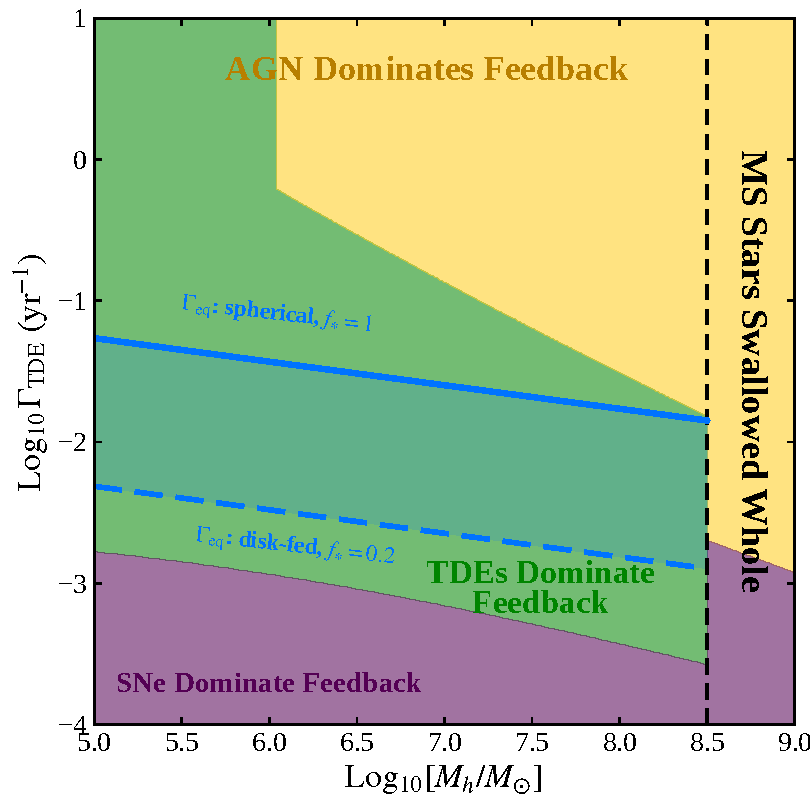
\includegraphics[width=0.4\linewidth,clip=true]{dominance.pdf}
\centering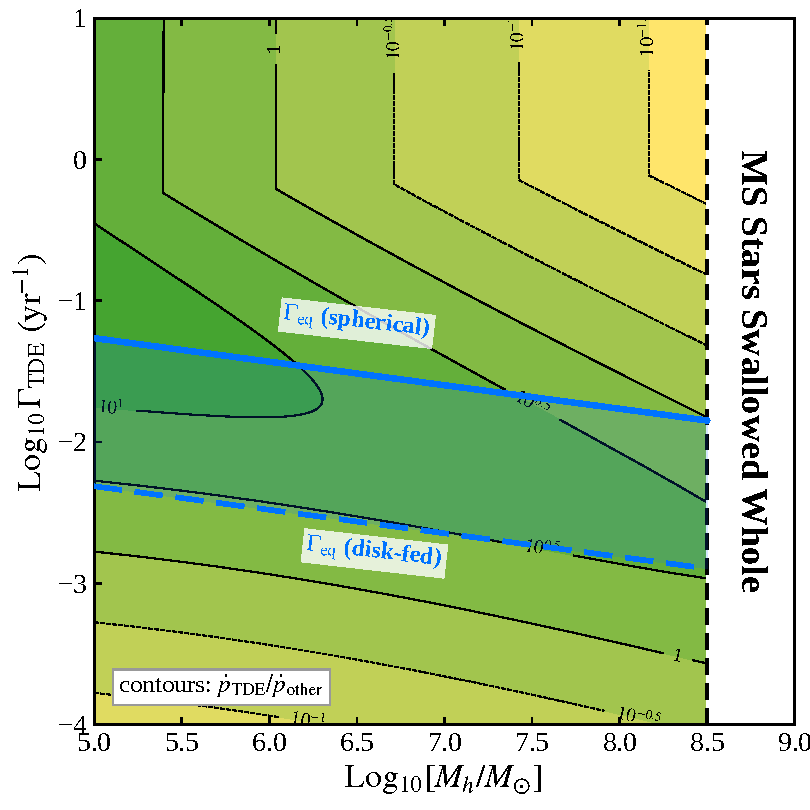
\includegraphics[width=0.4\linewidth,clip=true]{domratio.pdf}
\caption{Conditions under which tidal disruptions dominate all other sources of feedback in galactic nuclei. In the left-hand plot, the gold and green regions show where the AGN and TDE feedback mechanisms dominate for a given tidal disruption rate $\Gamma_{\rm TDE}$ and black hole mass $M_{\rm h}$. Within the region where TDEs dominate feedback, the equilibrium disruption rate relation \DIFdelbeginFL \DIFdelFL{, }\DIFdelendFL \DIFaddbeginFL \DIFaddFL{is represented by the blue lines: solid for the spherical solution of }\DIFaddendFL Equation (\DIFdelbeginFL \DIFdelFL{\ref{eq:eqrate}}\DIFdelendFL \DIFaddbeginFL \DIFaddFL{\ref{eq:eqrate}}\DIFaddendFL ), \DIFdelbeginFL \DIFdelFL{is represented }\DIFdelendFL \DIFaddbeginFL \DIFaddFL{dashed for the disk-fed solution of Section~\ref{subsec:disk} with $f_{\ast} = 0.2$, with the shaded band spanning the range $\Gamma_{\rm eq} \propto f_{\ast}^{3/2}$ allowed }\DIFaddendFL by the \DIFdelbeginFL \DIFdelFL{blue line}\DIFdelendFL \DIFaddbeginFL \DIFaddFL{geometry}\DIFaddendFL . The right hand plot shows the ratio of momentum injection from TDEs $\dot{p}_{\rm TDE}$ to that from all other momentum injection processes, $\dot{p}_{\rm other}$. If a system occupies any position within the green region, it will be driven towards the equilibrium line by adjusting $\Gamma_{\rm TDE}$.}
\label{fig:dominance}
\end{figure*}

\section{Starting and Stopping the Engine}\label{sec:spark}

As shown in Figure \ref{fig:dominance}, the minimum required disruption rate to sustain a disruption engine is $\gtrsim 10^{-4}$~yr$^{-1}$, and for some galaxies this rate might already be realized just from two-body relaxation \citep{Stone:2016a}. However, because of the dependence of the TDE momentum feedback on $M_{\rm h}$ (Equation (\ref{eq:pudr})), the $10^{-4}$~yr$^{-1}$ requirement is only sufficient for the most-massive black holes, $M_{\rm h} \gtrsim 10^{8} M_{\odot}$, such black holes tend to have longer relaxation times and thus lower rates of tidal disruption. For lower black hole masses the disruption rate requirements are stiffer, with $\gtrsim 10^{-3}$~yr$^{-1}$ likely being required for $10^{6} M_{\odot}$ black holes.

Once established, a disruption engine will maintain a high equilibrium rate so long as the galactic nucleus continues to be surrounded by molecular gas, and will naturally inhibit the local SNe rate and set the level of AGN activity. Thus, all that is required is to temporarily raise the disruption rate (``spark'' the engine) above the critical threshold necessary to enter into the disruption engine state. So long as this enhancement lasts for longer than the time it takes for massive stars to form and produce SNe ($\sim 5 \times 10^{7}$~yr$^{-1}$), the disruption engine will continue to operate even after the mechanism for the temporary increase stops operating.

A natural mechanism for temporarily enhancing the tidal disruption rate for a few $10^{8}$~yr is the merger of the black hole at the center of the nuclear cluster with a secondary black hole of comparable mass. Some models have predicted that such mergers can yield extremely high disruption rates \citep{Chen:2009a}, but even modest enhancements in the rate by a factor of $\sim 10$ above the nominal value can mean the difference between being in the self-sustaining engine state or not.

While it might seem natural to ascribe the rate increase predicted as the result of mergers with the observed rate enhancement, the primary issue is that the merger will only result in the disruption of a fixed number of stars that will be significantly less than the mass of the secondary black hole. The faster the merger, the higher the disruption rate, but at the expense of a shorter duration of enhancement. \citet{Wegg:2011a} estimate that only 3\% of all stellar disruptions come as the result of black hole mergers, a number that would need to be inverted (a few percent of disruptions around {\it single} black holes) to explain the observed enhancement.

If a black hole merger is responsible for sparking the engine, a plausible sequence of events that lead to a black hole being in the disruption engine state are:

\begin{enumerate}
\item Two galaxies merge, driving gas to the center of the more-massive galaxy. This yields a burst of star formation.
\item The two central black holes merge after 1 Gyr, enhancing the TDE rate. TDEs have the advantage that they accrete at rates much greater than Eddington, converting a larger fraction of the emergent energy into wide relativistic outflows.
\item The injection of kinetic energy suppresses star formation by \DIFdelbegin \DIFdel{destroying molecular clouds(need to find a reference that shows this)
}\DIFdelend \DIFaddbegin \DIFadd{sustaining turbulent support in the molecular clouds, in the same manner inferred for the Milky Way's Central Molecular Zone \mbox{%DIFAUXCMD
\citep{Longmore:2013a,Kruijssen:2014a}}\hskip0pt%DIFAUXCMD
.
}\DIFaddend \item \DIFdelbegin \DIFdel{These clouds push in to the Hill radius or closer, changing the transition from a full to an empty loss cone (Spitzer \& Schwarzschild, \mbox{%DIFAUXCMD
\citealt{Merritt:2013a}}\hskip0pt%DIFAUXCMD
, \mbox{%DIFAUXCMD
\citealt{Perets:2007a}}\hskip0pt%DIFAUXCMD
)}\DIFdelend \DIFaddbegin \DIFadd{The clouds settle into a belt close enough to act as massive perturbers, moving the nucleus from the empty toward the full loss cone regime \mbox{%DIFAUXCMD
\citep{Spitzer:1951a,Perets:2007a,Merritt:2013a}}\hskip0pt%DIFAUXCMD
}\DIFaddend .
\item The enhanced rate of TDEs maintains the suppressed star formation despite the massive gas reservoir. Enhanced TDEs continued until the gas reservoir is exhausted or ejected from the galaxy as a molecular outflow.
\end{enumerate}

\section{Discussion}\label{sec:discussion}

\subsection{\DIFdelbegin \DIFdel{Heating the rest }\DIFdelend \DIFaddbegin \DIFadd{The lifetime }\DIFaddend of \DIFdelbegin \DIFdel{the galaxy with the nuclear cluster}\DIFdelend \DIFaddbegin \DIFadd{an engine}\DIFaddend }\DIFaddbegin \label{subsec:lifetime}
\DIFaddend 

The \DIFdelbegin \DIFdel{amount of orbital energy being added to the nuclear cluster is comparable to the total binding energy of the stars in the galaxy}\DIFdelend \DIFaddbegin \DIFadd{engine is not perpetual: it consumes both the stars of the cusp and the gas of the disk. Disruptions remove stellar mass at a rate $m_{\ast}\Gamma_{\rm eq}$, so the cusp is exhausted in
}\begin{equation}
\DIFadd{t_{\rm cusp} = \frac{N_{\ast}}{\Gamma_{\rm eq}} = 1.2 \times 10^{9} \mhsix^{7/6}~}{\DIFadd{\rm yr}}\DIFadd{,
}\end{equation}
\DIFadd{while the disk, if it resupplies the cusp through star formation, is drained in
}\begin{equation}
\DIFadd{t_{\rm gas} = \frac{M_{\rm disk}}{m_{\ast} \Gamma_{\rm eq}} = 4.4 \times 10^{8} \mhsix^{1.3}~}{\DIFadd{\rm yr}}\DIFadd{,
}\end{equation}
\DIFadd{both evaluated for the disk-fed engine of Section~\ref{subsec:disk}. Gas exhaustion is the binding constraint, and it sets an engine lifetime of a few $10^{8}$~yr for a $10^{6}~\msun$ black hole, provided the disk is not replenished from larger radii. Since the circumnuclear reservoirs of post-starburst galaxies reach $\sim 10^{9}~\msun$, three orders of magnitude above the disk mass required here, resupply from outside is likely to extend this, and the cusp consumption time then becomes the ceiling.
}

\DIFadd{We note that these two timescales are close to one another in the spherical solution and separate by a factor of a few in the disk-fed one; their ratio is a diagnostic of the geometry rather than a robust prediction, and we caution against reading physical significance into the near-coincidence of the spherical case. What is robust is the order of magnitude: engines live for $10^{8}$--$10^{9}$~yr, neither so briefly that they would be vanishingly rare nor so long that they would be common. This overlaps the ages at which post-starburst spectral signatures are strongest, which offers a natural explanation for why TDE hosts are drawn so heavily from that population \mbox{%DIFAUXCMD
\citep{French:2020a,Hammerstein:2023a}}\hskip0pt%DIFAUXCMD
: the engine and the k+A signature are set by the same event and decay on comparable timescales.
}

\DIFadd{This also revises the expectation stated in Section~\ref{sec:intro} that the enhancement could persist for billions of years. Only the most massive engines approach that, and then only if their gas is continually replenished.
}

\subsection{\DIFadd{An obscured population of disruptions}}\label{subsec:obscured}

\DIFadd{The equilibrium ambient density implies a visual extinction $A_{\rm V} \simeq 50$ along a sightline that passes through the gas. A disruption seen through the clouds is therefore not a source that optical surveys can find: it is reprocessed by dust and emerges in the infrared}\DIFaddend .

\DIFdelbegin \DIFdel{See: Jeremy Goodman thermodynamic treatment of globular clusters
}\DIFdelend \DIFaddbegin \DIFadd{The obscuration is not isotropic, however, and this is where the disk geometry of Section~\ref{subsec:disk} makes a sharper prediction than the spherical belt. If the gas subtends only a fraction $f_{\Omega}$ of $4\pi$, then only that fraction of sightlines is extinguished; a nucleus viewed close to face-on offers an unobstructed view of the black hole even while an edge-on view is buried under $A_{\rm V} \simeq 50$. This is precisely the orientation dependence that underpins the unified model of active nuclei, in which the same object appears obscured or unobscured according to whether the torus intercepts the line of sight \mbox{%DIFAUXCMD
\citep{Netzer:2015a,RamosAlmeida:2017a}}\hskip0pt%DIFAUXCMD
.
}\DIFaddend 

\DIFaddbegin \DIFadd{The engine hypothesis therefore does not predict that all high-rate nuclei are hidden. It predicts that the obscured fraction of disruptions }{\it \DIFadd{equals the covering factor of the gas}}\DIFadd{, which for our fiducial $f_{\Omega} = 0.2$ means that roughly one engine disruption in five is lost to dust while the remainder are seen at close to their intrinsic brightness. This is a considerably more falsifiable statement than the spherical case, in which every sightline is blocked and the engine population would be invisible in the optical altogether. It also removes an obvious objection: were engines uniformly obscured, they could not contribute to the optically selected samples in which the post-starburst preference was found in the first place.
}

\DIFadd{This is a testable statement, and the evidence has moved in its favor since this work was begun. Mid-infrared searches have uncovered a population of dust-obscured disruptions whose hosts are gas-rich and star-forming, and which are largely invisible to optical surveys \mbox{%DIFAUXCMD
\citep{Masterson:2024a}}\hskip0pt%DIFAUXCMD
. The volumetric rates inferred from optical surveys \mbox{%DIFAUXCMD
\citep{vanVelzen:2021a,Yao:2023a} }\hskip0pt%DIFAUXCMD
fall short of loss-cone predictions by roughly an order of magnitude, which is the direction and approximate magnitude that a substantially obscured high-rate population would produce. We emphasize that the engine hypothesis does not require every obscured TDE to arise in an engine; it requires that nuclei with the highest rates be preferentially, but not exclusively, obscured. Measuring the ratio of infrared-selected to optically selected disruptions among post-starburst hosts would in principle measure $f_{\Omega}$ directly.
}

\DIFaddend \subsection{Rapid black hole growth through tidal disruptions}\DIFaddbegin \label{subsec:growth}

\DIFaddend For a Bondi fraction $f_{\rm B} = 10^{-3}$, Equation (\ref{eq:eqaccratio}) predicts that the rate at which matter is accreted by the black hole from tidal disruptions \DIFdelbegin \DIFdel{is approximately equal to the rate }\DIFdelend \DIFaddbegin \DIFadd{exceeds the rate at which }\DIFaddend it is acquired \DIFdelbegin \DIFdel{via accretion of }\DIFdelend \DIFaddbegin \DIFadd{from }\DIFaddend the ambient medium \DIFdelbegin \DIFdel{. However, this }\DIFdelend \DIFaddbegin \DIFadd{by a factor of a few for $M_{\rm h} \sim 10^{6}~\msun$, placing the engine in the ``black tide'' mode of growth \mbox{%DIFAUXCMD
\citep{Young:1977a}}\hskip0pt%DIFAUXCMD
. This conclusion is geometry-dependent: in the disk-fed engine of Section~\ref{subsec:disk} the same ratio is $0.25 f_{\rm B,-3}^{-1}$, and the ambient gas instead dominates unless the black hole is a relatively inefficient accretor. This }\DIFaddend ratio is entirely dependent on \DIFdelbegin \DIFdel{just }\DIFdelend how quickly the black hole accretes gas from the ambient medium; in cases where the accretion rate is closer to 1\% of Bondi \citep[e.g. M87,][]{Kuo:2014a}, the black hole's growth is still dominated by the accretion of the surrounding gas, whereas \DIFdelbegin \DIFdel{the }\DIFdelend \DIFaddbegin \DIFadd{a }\DIFaddend Bondi fraction of $\sim 10^{-4}$ \citep[e.g. the MW,][]{Quataert:2000a} would \DIFdelbegin \DIFdel{predict that TDEs would dominate black hole growth, \mbox{%DIFAUXCMD
\citep[the ``black tide'' model of black hole growth,][]{Young:1977a}}\hskip0pt%DIFAUXCMD
}\DIFdelend \DIFaddbegin \DIFadd{place growth firmly in the tidal channel. Because the accreted mass is delivered in discrete, super-Eddington episodes rather than continuously, the resulting duty cycle is highly intermittent, comparable to the flickering inferred for low-luminosity AGN \mbox{%DIFAUXCMD
\citep{Schawinski:2015a}}\hskip0pt%DIFAUXCMD
.
}

\DIFadd{Over an engine lifetime the black hole gains of order its own mass in stellar material in either geometry, since the lower disruption rate of the disk-fed solution is compensated by its longer lifetime. Engines are therefore not a negligible contribution to the growth of black holes in this mass range, though they are too rare to compete with radiatively efficient accretion in the global budget.
}

\subsection{\DIFadd{Suppressed star formation and the CMZ analogy}}\label{subsec:sf}

\DIFadd{The clouds are turbulently supported at ${\cal M} \simeq 40$ and sit at densities of $10^{4}$--$10^{5}~{\rm cm}^{-3}$ while forming few stars. This combination is unusual but not unprecedented: it is the condition of the Milky Way's Central Molecular Zone, where the star formation rate falls an order of magnitude below what the dense gas mass would predict \mbox{%DIFAUXCMD
\citep{Longmore:2013a,Kruijssen:2014a,Barnes:2017a}}\hskip0pt%DIFAUXCMD
. In the CMZ this suppression is generally attributed to the elevated turbulent pressure raising the density threshold for collapse; in an engine, the same suppression is maintained by UDR driving, and it is self-sustaining rather than incidental.
}

\DIFadd{The observational corollary is that engines should appear as nuclei rich in dense-gas tracers (HCN, HCO$^{+}$) but weak in star formation indicators, alongside a low level of AGN activity, $L_{\rm AGN}/L_{\rm Edd} \sim 0.06 f_{\rm B,-3}$. Such centrally concentrated, weakly star-forming molecular reservoirs are routinely observed in post-starburst galaxies \mbox{%DIFAUXCMD
\citep{Alatalo:2011a,Alatalo:2014a,Alatalo:2015a,French:2018a}}\hskip0pt%DIFAUXCMD
, which are the same hosts in which TDEs are over-represented}\DIFaddend .

\DIFdelbegin \subsection{\DIFdel{Observational implications}}
%DIFAUXCMD
\addtocounter{subsection}{-1}%DIFAUXCMD
\DIFdelend \DIFaddbegin \subsection{\DIFadd{Caveats}}\label{subsec:caveats}
\DIFaddend 

\DIFdelbegin \DIFdel{\mbox{%DIFAUXCMD
\citep{Schawinski:2015a}
}\hskip0pt%DIFAUXCMD
}\section{\DIFdel{Enhancement of k+A Galaxies in Clusters}}
%DIFAUXCMD
\addtocounter{section}{-1}%DIFAUXCMD
\DIFdelend \DIFaddbegin \DIFadd{The treatment here is deliberately an order-of-magnitude one, and several of its simplifications would need to be relaxed before the numbers above could be taken as predictions rather than as scalings.
}

\DIFadd{The most significant is the loss cone. We have adopted the full-loss-cone rate, justified by the presence of massive perturbers, but in the spherical solution the cusp stars sit near the boundary between the full and empty regimes ($q_{\ast} = 0.14 \mhsix^{-2/3}$), and the clouds are too distant to torque them directly. The disk-fed solution is better behaved in this respect ($q_{\ast} = 0.68 \mhsix^{-2/3}$), which is one of the reasons we prefer it, but neither case is comfortably deep in the pinhole regime for the most massive black holes considered. The rates we quote are thus upper envelopes. A direct $N$-body or Fokker-Planck treatment of a flattened cusp embedded in a massive-perturber disk would settle this, and would also test our assumption that the pinhole rate is insensitive to flattening while the collision rate is not; that asymmetry is what sets the scaling in Equation~(\ref{eq:gammaeqf}), and it deserves a more careful treatment than the scaling argument we have given it.
}

\DIFadd{We have also treated the clouds as a single population of identical objects at a single radius, ignored the dynamical friction that would cause them to spiral inward over $\sim 10^{9}$~yr, and adopted a single aspect ratio for both the gas and the stars, whereas a real nucleus would present a range of inclinations and a warped, possibly eccentric, disk. Each of these is a factor-of-a-few effect on quantities that already carry factor-of-a-few uncertainties, and none of them changes the central result: that a self-consistent, self-sustaining solution exists, that it lies a few hundred times above the canonical disruption rate, and that it is obscured.
}

\subsection{\DIFadd{Enhancement of k+A galaxies in clusters}}\label{subsec:ka}

\DIFaddend k+A galaxies show central molecular regions with a large amount of mass\DIFdelbegin \DIFdel{$\sim 10^{9} M_{\odot}$, }\DIFdelend \DIFaddbegin \DIFadd{, $\sim 10^{9}~\msun$, }\DIFaddend molecular outflows, and suppressed star formation \citep{Alatalo:2011a,Alatalo:2014a}. \DIFdelbegin \section{\DIFdel{Observational Signatures}}
%DIFAUXCMD
\addtocounter{section}{-1}%DIFAUXCMD
\subsection{\DIFdel{Dense molecular gas}}
%DIFAUXCMD
\addtocounter{subsection}{-1}%DIFAUXCMD
\subsection{\DIFdel{Suppressing star formation}}
%DIFAUXCMD
\addtocounter{subsection}{-1}%DIFAUXCMD
\begin{align*}
\DIFdel{n_{\rm crit} }&\DIFdel{= 9 \times 10^{6} \left(\frac{M_{\rm h}}{10^{7} M_{\odot}}\right)^{-1/2}~}{\DIFdel{\rm cm}}\DIFdel{^{-3}
}\end{align*}%DIFAUXCMD
\DIFdel{Looking for galaxies with dense tracers (e.g. HCN) with ALMA or CARMA. }\DIFdelend \DIFaddbegin \DIFadd{The disk mass required by the engine, $\sim 7 \times 10^{5} \mhsix^{1.14}~\msun$, is a small fraction of these reservoirs, so a k+A nucleus has ample fuel to sustain an engine for the $\sim 10^{8}$~yr derived above. The engine hypothesis therefore does not require these galaxies to be unusual in their total gas content, only in the configuration of the innermost few parsecs of it.
}\DIFaddend 

\DIFdelbegin \section{\DIFdel{Notes}}
%DIFAUXCMD
\addtocounter{section}{-1}%DIFAUXCMD
%DIFDELCMD < \begin{itemize}
\begin{itemize}%DIFAUXCMD
%DIFDELCMD < \item %%%
\item%DIFAUXCMD
\DIFdel{Explain why cosmic rays are likely not very important
}
\end{itemize}%DIFAUXCMD
%DIFDELCMD < \end{itemize}
%DIFDELCMD < %%%
\DIFdelend \DIFaddbegin \DIFadd{Three properties of the k+A population make them natural hosts. First, their morphologies are disturbed: a large fraction show tidal features and other signatures of a recent major merger \mbox{%DIFAUXCMD
\citep{Zabludoff:1996a}}\hskip0pt%DIFAUXCMD
, which supplies both the violent relaxation needed to spark the engine (Section~\ref{sec:spark}) and the inflow of gas needed to build the disk. Second, and less obviously, they retain that gas. Post-starburst galaxies were long assumed to have exhausted or expelled their molecular reservoirs, but sensitive CO and dust measurements find substantial cold gas surviving for hundreds of Myr after the burst \mbox{%DIFAUXCMD
\citep{French:2015a,Smercina:2018a}}\hskip0pt%DIFAUXCMD
. Third, that surviving gas is not forming stars at the rate its density would imply \mbox{%DIFAUXCMD
\citep{French:2018a}}\hskip0pt%DIFAUXCMD
, which is the same decoupling of dense gas from star formation that the engine requires and that the CMZ exhibits.
}\DIFaddend 

\DIFdelbegin \DIFdel{Metallicity enhancement reduced in galaxies with TDE feedback
}\DIFdelend \DIFaddbegin \DIFadd{Taken together, these are the conditions the model needs, and they are observed to persist on precisely the timescale over which we find an engine can run. We would add one caution: the causal arrow is not established by any of this. A merger that sparks an engine also produces a k+A spectrum and a central gas reservoir independently, so the association of TDEs with k+A hosts is equally consistent with the engine being a consequence of the same event rather than a cause of the elevated rate. Distinguishing the two requires the nuclear observations described above, not host-galaxy demographics.
}\DIFaddend 

\DIFdelbegin \DIFdel{Soltan argument
}%DIFDELCMD < 

%DIFDELCMD < %%%
\DIFdel{stark 1991 cloud dynamical friction
}%DIFDELCMD < 

%DIFDELCMD < %%%
\DIFdel{guesten 1987 molecular cloud disruption
}%DIFDELCMD < 

%DIFDELCMD < %%%
\DIFdel{ponti 2015 x-ray cones above/below GC
}%DIFDELCMD < 

%DIFDELCMD < %%%
\DIFdel{loeb and waxman cumulative neutrino background
}%DIFDELCMD < 

%DIFDELCMD < %%%
\DIFdel{battersby ``low SFR in MW center''
}%DIFDELCMD < 

%DIFDELCMD < %%%
\DIFdel{kjruijssen 2015
}%DIFDELCMD < 

%DIFDELCMD < %%%
\DIFdel{interacting disks from consecutive TDEs
}%DIFDELCMD < 

%DIFDELCMD < %%%
\DIFdel{\mbox{%DIFAUXCMD
\citep{Trouille:2013a}
}\hskip0pt%DIFAUXCMD
}%DIFDELCMD < \colr{Look at Fionna Harrisson's latest work, NuSTAR}
%DIFDELCMD < 

%DIFDELCMD < %%%
\DIFdelend \bigskip
\acknowledgements
We thank Fabio~Antonini, Blakesley~Burkhart, Xian~Chen, Charlie~Conroy, Robert~Fisher, Nathan~Goldbaum, Luke~Zoltan-Kelley, Morgan~MacLeod, Peter~Maksym, Ilya~Mandel, Michael~McCourt, Smadar~Naoz, Ryan~O'Leary, Enrico~Ramirez-Ruiz, Lorenzo~Sironi, and Nicholas~Stone for thoughtful discussions. This work was supported in part by Einstein grant PF3-140108 (J.~G.). J.~G. would like to thank the Aspen Center for Physics (NSF Grant \#1066293) for their generous hospitality\DIFaddbegin \DIFadd{. First paper draft was originally completed circa 2018; paper was updated in 2026 with the assistance of the Anthropic AI models Claude Fable and Opus 5. All references and AI edits were hand-checked by the authors}\DIFaddend .

\bibliographystyle{apj}
\bibliography{engineNotes}

\end{document}

